\documentclass[a4paper,12pt]{book}

\usepackage[utf8]{inputenc}
\usepackage[T1]{fontenc}
\usepackage[italian]{babel}
\usepackage[babel]{csquotes}

\usepackage{tocloft} 

\newcommand{\addappendixname}{% 
  \renewcommand{\cftchappresnum}{\appendixname\space}% 
    \settowidth{\cftchapnumwidth}{\bfseries \appendixname\space A\hspace{1em}}}

\usepackage{mathtools}
\usepackage{float}
\usepackage[center]{caption}

\usepackage{graphicx}
\usepackage{xcolor}

\usepackage{listings}
\addto\captionsitalian{\renewcommand{\lstlistingname}{Codice}}

\usepackage{setspace}
\onehalfspacing

\usepackage[square,comma,numbers,sort]{natbib}

\usepackage[fixlanguage]{babelbib}
\selectbiblanguage{italian}
\bibliographystyle{babplain-fl}

% biblio in inglese ?
%\bibliographystyle{plain}

\usepackage[breaklinks]{hyperref}
\hypersetup{
	colorlinks,
  citecolor=black,
  filecolor=black,
  linkcolor=black,
  urlcolor=black
}
\usepackage[all]{hypcap}


\begin{document}

\begin{titlepage}

\begin{center}
\large
\textsc{\Large Università degli Studi di Pisa\\}
\vspace{0.2cm}

\includegraphics[width=2.8cm]{img/logo_unipi.pdf}

\vspace{0.2cm}
\textsc{\large Facoltà di Scienze Matematiche, Fisiche e Naturali}\\ \vspace{0.1cm}

\textsc{\Large{Corso di Laurea Triennale in Informatica}}\\

\vspace{3cm}

{\Huge\textbf{L7-Bridge}}\\[0.2cm]
{\Large{Un firewall applicativo per il riconoscimento\\dei servizi Internet}}\\[0.2cm]

\vspace{6cm}

\begin{minipage}{0.45\linewidth}
\begin{center}
{\Large Candidato\\} \vspace{0.07cm} \textbf{{\Large Jacopo Lipilini}}\\
\vspace{-0.0cm} {\normalsize \ttfamily jacopo.lipilini@gmail.com}
\end{center}
\end{minipage}
\hfill
\begin{minipage}{0.45\linewidth}
\begin{center}
{\Large Docente e Tutore\\} \vspace{0.07cm} \textbf{{\Large Prof. Luca Deri}}\\
\vspace{-0.0cm} {\normalsize \ttfamily deri@ntop.org}
\end{center}
\end{minipage}

\end{center}

\end{titlepage}

\clearpage{\pagestyle{empty}\cleardoublepage}
\pagenumbering{roman}
\pagestyle{plain}
\tableofcontents


\mainmatter
\pagenumbering{arabic}
\pagestyle{headings}
\clearpage{\pagestyle{empty}\cleardoublepage}
\chapter{Introduzione}

\section{Uno sguardo d'insieme}

Internet nacque verso la fine degli anni sessanta grazie ad un progetto militare statunitense. Allora si chiamava Arpanet ed era il prototipo di un nuovo sistema di difesa e di controspionaggio ideato nell'ambito della Guerra Fredda. All'atto della sua creazione, pochi importanti nodi del Nord America erano connessi tra loro e le linee di collegamento trasportavano semplici informazioni testuali a bassissime velocità.

Al giorno d'oggi, grazie al progresso della tecnologia, che ha introdotto nel mercato apparecchiature di rete e PC a prezzi modici, e della globalizzazione, che li ha portati in ogni angolo del pianeta, Internet è diventata la \emph{rete delle reti} e connette tra loro miliardi di utenti in tutto il mondo. Consentendo lo scambio a notevole velocità di contenuti anche piuttosto complessi come foto, filmati, videogame \dots , è il principale mezzo di comunicazione di massa. Tale aspetto è evidenziato anche in campo economico dal fatto che spesso le aziende vi si affacciano al fine di offrire nuovi ed innovativi servizi. Basti pensare all'ascesa nel panorama mondiale che stanno avendo Facebook, Twitter e YouTube, piuttosto che eBay.

Le risorse di rete non sono però illimitate e inoltre sono condivise da un numero sempre più elevato di utilizzatori, sia attraverso i computer che tramite l'uso dei cellulari di ultima generazione. Quindi è ovvio che bisogna sfruttare al meglio quelle disponibili. Di conseguenza, si ha la necessità di garantire agli utenti un certo livello di qualità di determinati servizi e allo stesso tempo di limitarne altri. Per esempio un negozio potrebbe volere che dai propri PC sia possibile comunicare celermente con il magazzino centrale, ed evitare che i propri dipendenti perdano tempo a guardare video su YouTube.

In risposta a questa esigenza, cominciarono ad essere elaborati dei programmi in grado di bloccare le comunicazioni indesiderate, i \emph{firewall}.

Queste applicazioni, fatte girare su macchine poste al confine tra una rete e l'altra, esaminano le informazioni in transito e prendono decisioni (se permettere o meno la comunicazione) basandosi sulla natura del traffico di dati.

L'evoluzione informatica, la facilità con cui ognuno può aggiungere funzionalità alla rete senza dover seguire un rigido processo di standardizzazione e la semplicità con cui si possono modificare (e falsificare) le informazioni, han però fatto sì che presto tali programmi restassero indietro rispetto al progresso di Internet, diventando quindi piuttosto obsoleti. Di fatto, data la grande possibilità di personalizzazione, non esistono più regole semplici ed immediate sulle quali basarsi.

C'è quindi bisogno di ripensare la struttura dei firewall per renderli più adatti alle reti attuali. Nasce così il progetto \emph{L7-Bridge}.

\section{Il progetto L7-Bridge}

Questo progetto si propone di rendere il firewall, componente ormai essenziale di ogni rete, in grado di ispezionare più approfonditamente il traffico al fine di riconoscere quale servizio (anche detto \emph{protocollo applicativo}) sta effettivamente utilizzando le risorse, ovviamente senza costituire esso stesso un elemento di rallentamento. Sarebbe infatti inutile avere un sistema che impieghi così tanto tempo per elaborare un pacchetto da rendere lentissima, o addirittura inutilizzabile, una rete, seppur all'avanguardia tecnologicamente e capace di trasportare grandissime quantità di dati.

In questo caso ci viene in aiuto la continua corsa dei produttori di processori nel realizzare CPU sempre più performanti, in grado di eseguire svariati miliardi di operazioni al secondo e quindi, in nostri termini, di processare moltissime informazioni.

Inoltre le astrazioni informatiche permettono, oltre a processare (virtualmente) in contemporanea più informazioni, anche dei meccanismi per catturarle dalla rete ad alta velocità per portarli direttamente al motore d'analisi del firewall, consentendo un'ulteriore accelerazione dell'elaborazione.

Insomma, le premesse ci sono tutte per rendere molto interessante muoversi in questa direzione, al fine di sviluppare un prodotto innovativo che potrà colmare il gap tra l'espansione dei servizi Internet e l'attuale concezione del firewall.

Gli amministratori di rete, per esempio, avranno a disposizione un programma flessibile, facilmente configurabile e aggiornabile, da poter utilizzare ogniqualvolta abbiano la necessità di filtrare certo traffico per garantire priorità a determinati protocolli applicativi e scoraggiare, o anche impedire, l'uso di altri.

Ovviamente tale obiettivo può essere raggiunto solo se la macchina ospitante l'applicazione è posta sul confine tra una rete e l'altra senza che vi sia possibilità di far passare il traffico attraverso altre postazioni da e verso l'esterno. Così facendo si ottiene un controllo totale sui flussi di comunicazione, garantendo una piena operatività dei filtri. Ne risulta quindi che l'ubicazione perfetta sia ad esempio in un PC con due schede di rete. Una sul lato della rete interna da sorvegliare, e l'altra sul lato del resto del mondo (come illustrato in figura \ref{ubifw}). Tale configurazione prende, in gergo di rete, il nome di \emph{bridge}.

Naturalmente è da qui, e dal proposito di riconoscere i protocolli applicativi (che sono concettualmente al livello 7 del modello ISO/OSI), che il progetto deve il suo nome.

\begin{figure}[!htbp] % H !htbp
\begin{center}
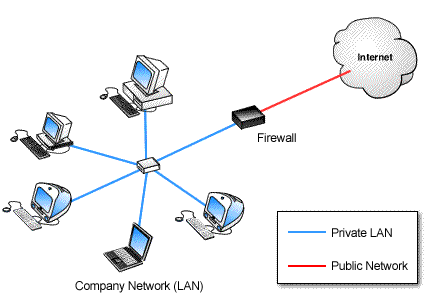
\includegraphics[scale=0.5]{img/ubicazione_fw.png}
\caption{Esempio di ubicazione del firewall}\label{ubifw}
\end{center}
\end{figure}

Lo sviluppo del codice è avvenuto in totale autonomia. Non sono comunque mancati l'appoggio e i suggerimenti preziosi del professore, che, data la sua esperienza nel campo del monitoraggio di reti ad alte prestazioni, hanno consentito un soddisfacente raggiungimento degli obiettivi preposti, con diverse possibilità di ampliamento futuro.

Anche grazie ad incontri appositi piuttosto costruttivi col professore per scambi di idee e pareri, sono state approfondite le conoscenze sui vari aspetti che riguardano la programmazione di rete, con particolare attenzione alle performance, aspetto centrale del progresso tecnologico.

%\clearpage

\section{Struttura della relazione di tirocinio}
{{\samepage
La relazione di tirocinio si articola su altri cinque capitoli, oltre a questo di carattere generale e introduttivo.
\begin{description}
\item[Capitolo 2] Dettaglio delle motivazioni, degli obiettivi e degli aspetti centrali del progetto.
\item[Capitolo 3] Implementazione scelta per risolvere il problema.
\item[Capitolo 4] Validazione e test a cui il sistema è stato sottoposto.
\item[Capitolo 5] Le altre soluzioni che ora il mercato mette a disposizione.
\item[Capitolo 6] Conclusioni a cui si è arrivati a seguito della realizzazione di questo progetto.
\end{description}
}}
\clearpage{\pagestyle{empty}\cleardoublepage}
\chapter{Progettazione}

\section{Le motivazioni del progetto}

Dall'introduzione sono emersi due aspetti centrali e imprescindibili per i firewall di nuova generazione, che saranno trattati in dettaglio nel proseguo di questo capitolo.

Il primo è la necessità di esaminare i pacchetti approfonditamente (DPI), senza soffermarsi all'header, poiché non è possibile in alcun modo fare un mappatura 1 a 1 delle porte coi servizi trasportati, sia per la continua espansione di quest'ultimi, che per la facilità nella manipolazione dei pacchetti.

Il secondo riguarda lo shaping, ovvero la gestione, attraverso politiche prestabilite, delle (limitate) risorse di rete, dato che sempre più device (cellulari, tablet, PC, \dots) possono accedervi, e potenzialmente monopolizzare la banda per servizi secondari a discapito di quelli primari.

Allo stato attuale, i due aspetti sono fondamentalmente disgiunti. Purtroppo, mantenerli separati ha notevoli implicazioni nelle veloci reti moderne, che, al contrario, richiedono grande collaborazione e integrazione tra DPI e shaping, al fine di garantire la miglior esperienza utente possibile.

Per quanto l'aspetto modulare sia una caratteristica desiderabile, averla tra tool completamente diversi e a sé stanti, che invece dovrebbero formare un unico sistema, non la è affatto.

Gli amministratori di rete sono quindi praticamente costretti a scegliere i costosi prodotti proprietari al fine di ottenere firewall aggiornati e performanti, adatti alle reti attuali. Le poche alternative open source, capaci di funzionare su hardware non dedicato e quindi meno costosi (ad esempio una workstation), spesso non forniscono l'integrazione di funzionalità ormai base come il DPI e lo shaping.

Per cercare di creare un sistema in grado di combinare i due aspetti, gli amministratori di rete sono costretti a provare a far interagire programmi di diversa natura. Ci sono quindi evidenti problemi derivati dalla comunicazione e dalle configurazioni da mantenere coerenti tra vari processi. Soprattutto queste ultime sono difficilmente gestibili in grosse realtà, dove spesso ci si trova a dover aggiornare un grande e complicato sistema.

Queste difficoltà sfociano nell'impossibilità di avere un controllo totale sul traffico, sia perché avere questa distribuzione di funzionalità forzata fa sì che i vari controlli siano più facilmente superabili (magari a causa proprio di una cattiva interoperabilità), sia a causa di un degradamento delle performance, richieste sempre più elevate dalla sempre crescente velocità delle reti.

Ne consegue il bisogno di accentrare in un unico software tutte le componenti necessarie a svolgere le funzioni di DPI e shaping, pur mantenendo l'aspetto buono della modularizzazione.

La voglia di modernizzare il mondo dei firewall, portandolo al passo con le reti attuali, ha fatto sì che questo progetto integrasse assieme tutti questi aspetti, al fine di portare, nel palcoscenico dei software di rete odierno, una grande novità.

Data la scarsità, o meglio, assenza, di prodotti simili nel mondo open source, si è deciso di colmare questo vuoto, fornendo quindi a tutti la possibilità di utilizzare al meglio le proprie risorse di rete, senza aver la necessità di star dietro alle sempre nuove tecnologie che quotidianamente vengono messe in commercio.

Ci si prefigge quindi l'obiettivo di creare un firewall a livello applicativo di nuova concezione, facilmente portabile e configurabile, capace di adattarsi perfettamente all'hardware sottostante (seppur di un semplice PC) per sfruttare al meglio la potenza di calcolo, così da offrire sul mercato un nuovo e valido strumento per gli amministratori di rete.

Quest'ultimi avranno anche la possibilità di scrivere le proprie funzioni per il riconoscimento dei protocolli applicativi, garantendo quindi un altissimo grado di personalizzazione.

Grazie alla tecnologia attuale, gli apparati di rete sono in grado di gestire traffico a velocità intorno al Gigabit/s, quindi il firewall viene concepito e realizzato per rispondere a questa esigenza.

Anche per questioni legate alla sicurezza, il sistema opera in modo del tutto trasparente, cioè come se fosse invisibile sia ai device interni che esterni.

\emph{L7-Bridge}, rispondendo a tutte queste prerogative, costituisce la prima concreta alternativa open source per il mondo firewall di ultima generazione.

\section{Principali problemi affrontati}

\subsection{Il Deep Packet Inspection}

Un componente fondamentale della nuova concezione di un firewall sta in un motore di analisi approfondita dei pacchetti \cite{dpi} (in inglese \emph{Deep Packet Inspection}, in sigla DPI), dato che i numeri di porta non identificano più i servizi Internet. Inoltre sempre più spesso il traffico viene criptato per favorire l'aspetto della sicurezza nella comunicazione.

Tale motore permette di non soffermarsi all'intestazione di un pacchetto in transito, ma di analizzarne approfonditamente anche il contenuto (\emph{payload}) al fine di capire cosa realmente sta trasportando. Questo avviene sia a livello di singolo pacchetto, dove interviene ovviamente la conoscenza del protocollo stesso (per esempio si sa che una risposta del protocollo di trasferimento file, FTP, inizia sempre con un codice di tre numeri seguiti da una breve stringa di spiegazione di quel codice), che dell'intero flusso di dati. Infatti spesso c'è bisogno di una sorta di memoria dei precedenti pacchetti transitati sia a fini statistici e di monitoraggio della rete, che al fine di stabilirne il servizio trasportato.

Si capisce quindi come sia necessario mantenere in memoria una struttura dati per contenere tali informazioni e che ne permetta un rapido accesso al fine di non rallentare le operazioni di ispezione del pacchetto.

Spesso, congiuntamente all'analisi, è anche possibile estrarre altre varie informazioni sul traffico (\emph{metadati}).

I metadati possono essere utilizzati al fine di tracciare dei veri e propri profili d'uso sia a livello della rete nel complesso che a livello dei singoli utenti.

Questo meccanismo è sfruttato anche dagli ISP (Internet Service Provider, ovvero in italiano, il fornitore dei servizi Internet) a fini commerciali. Se tale pratica sia o meno corretta dipende, oltre che dal buonsenso, anche dalla legislazione di ogni stato.

Infine, il DPI consente anche di riconoscere certi attacchi informatici come quelli dovuti a virus e worms, garantendo quindi un certo grado di sicurezza, altro aspetto fondamentale di un buon firewall.

Ci sono però degli svantaggi nell'usare questa tecnologia.

Dal punto di vista computazionale, si nota sicuramente come tutto ciò voglia dire spendere svariate operazioni per ogni pacchetto al fine di riconoscerne il protocollo applicativo e su reti ad alta velocità (Gigabit Ethernet per esempio) questo potrebbe voler dire perdere dei dati, in quanto sulla scheda continuano ad arrivare pacchetti che verrebbero poi scartati dalla scheda stessa per quelli più nuovi al termine dello spazio disponibile nel buffer temporaneo di memorizzazione.

Dal punto di vista dell'utente invece, questi meccanismi potrebbero essere visti come un attentato alla sua privacy.

Ad ogni modo, se utilizzato per giusti scopi, il DPI promette di essere il futuro per ogni firewall che si rispetti e un campo di ricerca in costante evoluzione, al pari dei servizi Internet.

Nel mercato mondiale, vi sono diversi prodotti software che svolgono questi compiti. Alcuni si appoggiano all'uso delle espressioni regolari, altri all'uso di funzioni C, per ispezionare i pacchetti.

L'utilizzo di espressioni regolari permette una semplice e intuitiva scrittura di nuovi pattern per riconoscere il protocollo applicativo del pacchetto, mentre le funzioni C permettono migliori performance dal punto di vista computazionale, a discapito della potenza espressiva. Inoltre, altro aspetto da non trascurare, le espressioni regolari sono più soggette ad effettuare errori nel match del servizio, creando quindi delle possibilità concrete di falsi positivi e negativi, caratteristica poco apprezzabile.

Al fine di colmare questi gap nei confronti delle funzioni C, sono stati compiuti, negli ultimi anni diversi, diversi studi \cite{redpi0,redpi1,redpi2,redpi3}. Congiungendo i vari risultati, si potrebbero ottenere ottime performance, con controlli paralleli di più espressioni e minor occupazione di memoria, accompagnate da un netto abbassamento delle probabilità di errori nel match.

I software migliori e più aggiornati risultano essere quelli a pagamento (piuttosto cara ogni licenza), ma essendo closed source c'è bisogno di attendere gli aggiornamenti voluti dai proprietari del software, che potrebbero non essere in linea con le esigenze dell'utente. La controparte open source invece, oltre che essere spesso inefficiente, è anche poco aggiornata e aggiornabile.

Oltre a prodotti software, ci sono soluzioni integrate in appositi apparati di rete. Essendo tecnologie all'avanguardia sono però piuttosto costose, e per ottenere aggiornamenti bisogna attendere quelli della casa produttrice.

In teoria questa soluzione è preferibile nei confronti di quelle software da far girare su comuni PC, in quanto, sfruttando unità specializzate, possono ottenere performance migliori, subordinate però, oltre che alla frequenza nell'aggiornamento, anche all'avanzamento delle tecnologie.

\subsection{Il Quality of Service}

Il Quality of Service \cite{qos} (Qualità del Servizio) e lo Shaping \cite{ts} (letteralmente, sagomatura) sono altri due aspetti fondamentali nell'attribuzione prioritaria delle risorse di rete, che, come detto, sono limitate.

Il tutto si traduce nell'assegnare una priorità ai flussi di comunicazione, e quindi, in accordo con esse, di ritardare certi pacchetti per favorire l'invio di altri, facendo in modo da destinare una maggior o minor quantità di risorse di rete.

Ovviamente tali risorse sono attribuite in base a quelle effettivamente disponibili, ma anche secondo le preferenze dell'utente o amministratore di rete che sia, configurando opportunamente il sistema che effettua lo shaping.

\clearpage
Da un punto di vista pratico, una volta che il traffico arriva al sistema, ad esso viene assegnato un grado di priorità, che manterrà per tutta la durata della comunicazione. I pacchetti che compongono il flusso non vengono immediatamente trasmessi all'altro capo, ma piuttosto vengono trattenuti per un certo periodo di tempo, al fine di dare precedenza a quelli a priorità maggiore.

Tutto ciò è dunque molto importante, oltre che per ottimizzare l'uso della rete nel suo complesso, anche per garantire a determinati utenti le migliori prestazioni possibili per certi servizi, sia sulla base di semplici preferenze che di accordi economici.

Lo svantaggio di questa tecnica è l'introduzione di un ulteriore livello di ritardo dal punto di vista computazionale, seppur fisiologico. I pacchetti candidati alla trasmissione devono essere memorizzati per tutto il tempo necessario in un buffer dell'applicazione che non può essere illimitato, quindi ancora una volta ci si potrebbe ritrovare a perdere dei pacchetti.

Nonostante tutto, attribuire a determinati servizi delle risorse minime da poter utilizzare per garantire l'usabilità dei sistemi da parte degli utenti, è una prerogativa troppo importante per essere ignorata.

Può essere effettuato sia su IP e porte, che sul protocollo applicativo realmente trasportato.

Nel primo caso il compito si esegue esaminando l'header del pacchetto e quindi praticamente a costo zero (c'è solo la decodifica del pacchetto). Nel secondo, invece, c'è anche la necessità di appoggiarsi ad un motore d'analisi DPI come quelli precedentemente discussi.

Esistono fondamentalmente due algoritmi per modellare il traffico. Uno è il \emph{leaky bucket} \cite{lba} e l'altro è il \emph{token bucket} \cite{tba}.

Seppur siano preposti allo stesso scopo, hanno caratteristiche diverse nel comportamento, infatti, mentre il primo impone un limite rigido sulla velocità di trasmissione dati, il secondo consente qualche picco ma il tasso medio di trasmissione risulta essere quello desiderato.

In questo caso è possibile utilizzare soprattutto soluzioni software, commerciali e open source.

I prodotti commerciali soffrono di tutte le varie pecche dei software closed source (alto prezzo e aggiornamento imposto).

I prodotti open source per Windows sono basati su algoritmi di shaping del tipo di quelli suddetti. Nel mondo di Linux invece abbiamo diversi approcci per risolvere questo problema, oltre a quello puramente algoritmico, il che li rende decisamente più interessanti.

Il più comune è quello che si basa su varie manipolazioni del \emph{traffic control} del kernel di Linux \cite{lntc} (un'esaustiva e aggiornata guida di come sia possibile utilizzarlo a fini di \emph{traffic shaping} si trova qui \cite{lartc}).

La prima cosa che salta allo sguardo è come questi meccanismi siano tutt'altro che semplici ed intuitivi, e la forte dipendenza dal kernel di Linux. Questo aspetto fa sì che si debbano adeguare sempre e costantemente alle varie modifiche che subiscono frequentemente i kernel, cosa che può diventare piuttosto inaccettabile.

Risulta quindi evidente come tali software siano destinati a non avere grande futuro, a meno di costanti revisioni.

Un altro approccio consiste nell'interporsi tra le  normali system calls chiamate dal programma (quali poll, select, recv, send, \dots) ritardandone eventualmente la reale esecuzione. Questo è fatto attraverso l'uso di LD\_PRELOAD sui sistemi Unix-like, che garantisce la precedenza di caricamento a certe librerie, a discapito di quelle standard come \emph{libc.so}.

Tramite questo accorgimento, piuttosto semplice, è possibile quindi limitare la banda di un'applicazione.

La terza possibilità è rappresentata dai \emph{packet scheduler}.

Questi possono essere implementati sia a livello utente che in kernel space.

Il compito dello scheduler è quello di dare un ordine per la spedizione ai vari pacchetti privilegiando quelli che rispettano determinati parametri, in modo da garantire una certa qualità di servizio.

Esistono vari tipi di politiche di scheduling, ognuna con le proprie caratteristiche. Una panoramica piuttosto esaustiva è contenuta in \cite{ps}.
\clearpage{\pagestyle{empty}\cleardoublepage}
\chapter{Implementazione}

\section{Le scelte di base}

La primissima scelta che ci si pone davanti è chiaramente quella sul linguaggio di programmazione da adottare. Siccome tutte le premesse fatte hanno come denominatore comune la \emph{velocità} nell'esecuzione delle varie operazioni, si sono scelti il C e il C++, che essendo linguaggi compilati offrono sicuramente prestazioni migliori rispetto a linguaggi interpretati. Inoltre, la prerogativa di realizzare un software libero, suggerisce di sviluppare il programma su Linux, il sistema operativo libero per antonomasia.

Facciamo un piccolo riassunto di cosa macroscopicamente il firewall debba fare. Per prima cosa, bisogna catturare il pacchetto dalla scheda di rete, successivamente processarlo, salvando le informazioni utili e analizzandolo completamente per riconoscerne il protocollo applicativo, ed infine, decidere se e quando trasmetterlo sull'altro lato.

Per rispondere alla prima esigenza è stata naturalmente presa in considerazione la classica libreria PCAP \cite{pcap,pcap2}. Purtroppo tale libreria è stata ideata in un momento in cui le schede di rete erano decisamente più lente, quindi risulta inadeguata ai nostri scopi. Così si è optato per l'utilizzo della libreria PF\_RING \cite{pfring}, che garantisce un rate di cattura intorno al Gigabit/s.

Per processare il pacchetto sono necessarie due operazioni. La prima consiste nel salvare in un'apposita struttura dati le varie informazioni che via via si ricavano dai pacchetti catturati. Dal corso di Algoritmica, risulta subito chiaro come l'utilizzo di una hash table di dimensione statiche (per evitare il blocco dell'esecuzione per attendere il ridimensionamento) con collisioni gestite a lista di trabocco sia la soluzione migliore in termini di prestazioni. La seconda, di importanza centrale nel firewall, analizza il pacchetto ricevuto fino al payload trasportato. Pochissime librerie open source consentono di eseguire il DPI efficientemente. La libreria L7-Filter \cite{l7filter}, eseguendo il confronto per pattern matching di espressioni regolari, è piuttosto lenta, e soffre dei problemi legati ai falsi positivi. Quindi la scelta è ricaduta sulla libreria nDPI \cite{ndpi}, che utilizzando semplici funzioni C permette prestazioni superiori e una probabilità di errore nel riconoscimento del protocollo applicativo praticamente nulla.

Infine il firewall si trova a dover affrontare una scelta, se far proseguire il pacchetto verso la destinazione o meno. A questo punto si consultano le regole impostate dall'utente salvate anch'esse in un'apposita struttura dati. In questo caso, la tabella hash non è la soluzione indicata, in quanto comunque le regole vanno scelte anche in base al prefisso più lungo comune sull'indirizzo IP. Sempre dal corso di Algoritmica, la miglior struttura dati da usare in questo caso risulta essere un albero binario sui bit dell'indirizzo.

\subsection{I PF\_RING}

I PF\_RING \cite{pfring} non sono altro che un nuovo tipo di socket di rete in grado di catturare pacchetti dalla scheda di rete e portarli in spazio utente, riuscendo a gestire traffico a velocità anche intorno ai 10 Gigabit/s.

L'idea alla base di questa tecnologia è quella di utilizzare un buffer circolare (detto \emph{ring}) dove salvare i pacchetti ricevuti dalla scheda e quindi passare all'applicazione il puntatore al pacchetto tramite una chiamata alla system call mmap(), mappando cioè in memoria virtuale del programma tale indirizzo. Questo è ottenuto attraverso due strati di polling. Uno posto tra la scheda e il \emph{ring}, l'altro tra il \emph{ring} e l'applicazione. Il primo sfrutta le NAPI (o New API) \cite{napi}, delle tecniche che consentono di mitigare l'effetto degli interrupt del device sul kernel di Linux, potendo richiederne l'intervento dopo un certo numero di pacchetti ricevuti (infatti il comportamento standard impone che ogni volta che la scheda riceva un pacchetto, mandi un \emph{interrupt} al sistema operativo per richiederne l'elaborazione, interrompendone quindi continuamente l'esecuzione). Il secondo sfrutta un semplice meccanismo di polling dei vari \emph{ring}, al fine di trovare nuovi pacchetti da portare in user-space tramite la funzione mmap().

Una peculiarità è l'indipendenza dallo specifico driver della scheda di rete. Vi sono tuttavia una serie di driver riscritti per supportare la vera potenza dei PF\_RING, i DNA driver.

Il DNA (\emph{Direct NIC Access}) \cite{pfringdna} consente di accedere direttamente alla memoria della scheda di rete, mappandone gli indirizzi. Potendo fare questo tipo di accesso ai vari registri del device, non c'è più bisogno di utilizzare la CPU. Si ha un grande miglioramento delle performance dovuto sia al risparmio dei cicli di clock spesi per salvare il pacchetto nel \emph{ring}, che quelli spesi per interrogare il device sui nuovi pacchetti ricevuti. Ciò che viene sfruttato ora, è la NPU (\emph{Network Processing Unit}), al fine di portare il pacchetto dalla scheda al \emph{ring} aperto in modalità DMA (\emph{Direct Memory Access}). Il risultato di tutto questo, è la possibilità di inviare e ricevere pacchetti di qualsiasi grandezza alla stessa velocità supportata dalla scheda.

\begin{figure}[htbp]
\begin{center}
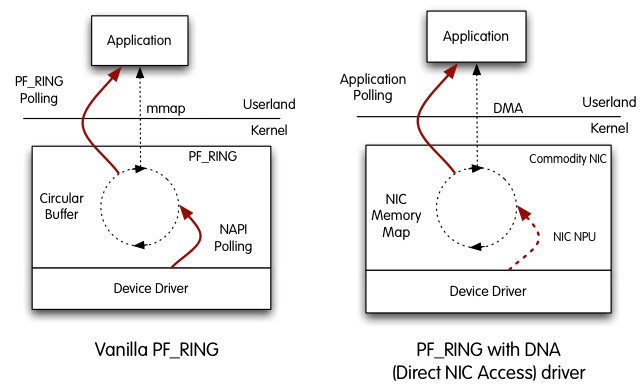
\includegraphics[scale=0.5]{img/PF_Ring_DNA.png}
\caption{Confronto tra le due realizzazioni}\label{PFRingDNA}
\end{center}
\end{figure}

\subsection{La libreria nDPI}

Per affrontare il problema cardine del nuovo concetto di firewall, ovvero l'analisi approfondita dei pacchetti, è stata scelta la libreria nDPI \cite{ndpi}, scritta in C, e nata dalle ceneri di un altro progetto open source abbandonato, \emph{OpenDPI}, del quale sul web rimangono pochissime tracce.

Data la sua natura, oltre a ottime performance, garantisce una quasi inesistente possibilità di avere dei falsi positivi e negativi, caratteristiche davvero importanti per una libreria che si occupa del DPI.

Questa libreria permette di esaminare singoli pacchetti, tenendo conto anche delle informazioni precedentemente salvate su quel flusso (reperibili dalla hash table), al fine di ottenere un codice identificativo del protocollo applicativo. Se nessuna corrispondenza venisse trovata col primo pacchetto, si dovrebbe procedere con i successivi che via via arriveranno al sistema, al fine di trovarne il servizio effettivamente trasportato.

Purtroppo non è sempre possibile risalire al protocollo applicativo (ad esempio perché tale protocollo non è supportato dalla libreria, oppure perché è cambiato nel tempo). Quindi conviene provare ad identificare il flusso solo per un numero di pacchetti limitato, per non incorrere in inutili prove, costose in termini di tempo. Dopodiché, se non si trovasse il servizio trasportato, tale flusso rimarrebbe non riconosciuto.

I protocolli riconosciuti sono comunque circa 150 e comprendono servizi usati per le funzioni di connettività e utilità (come DNS, DHCP, TELNET, NETBIOS, \dots), mail (POP3, SMTP, IMAP, GMAIL, \dots), web (HTTP, Flash, QuickTime, FaceBook, Twitter, YouTube, \dots), giochi e simili (Quake, SecondLife, \dots), trasferimento file (FTP, EDonkey, BitTorrent, \dots), \dots . Insomma, un parco protocolli davvero completo in grado di spaziare tra i vari settori d'uso di Internet.

Per eseguire le sue operazioni, tutte le chiamate a funzione fanno capo ad un'unica struttura principale condivisa che ha al suo interno, fra le altre cose, un buffer di funzioni. Queste sono quelle che realmente provano a stabilire se un dato pacchetto, passato come argomento, appartiene ad un certo protocollo applicativo.

Risulta quindi evidente come questa libreria sia facilmente estendibile. Basterà aggiungere a tale buffer una nuova funzione per identificare un nuovo protocollo (codificato da un numero univoco rispetto agli altri), per avere un nuovo servizio supportato.

Anche questo aspetto di flessibilità e facilità nell'aggiornamento è stato determinante per la scelta di questa libreria.

\subsection{L'architettura del sistema}

\begin{figure}[htbp]
\begin{center}
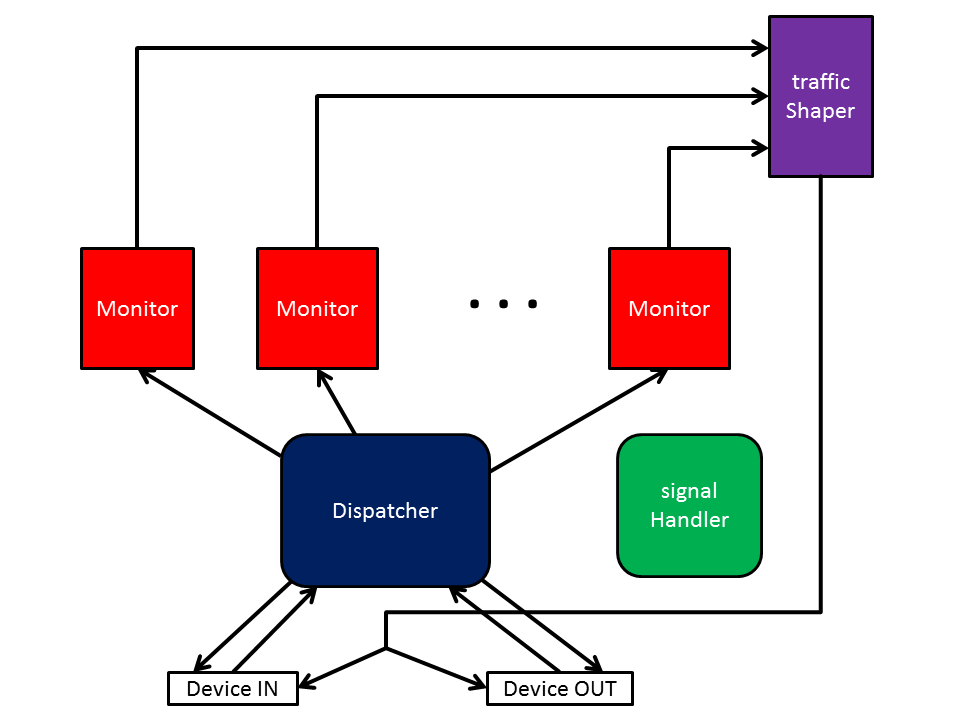
\includegraphics[scale=0.5]{img/arch.png}
\caption{L'architettura del sistema}\label{arch}
\end{center}
\end{figure}

Come si evince dalle considerazioni precedenti, c'è bisogno di una buona potenza di calcolo al fine di gestire grosse quantità di pacchetti.

Poiché l'elaborazione è in un certo senso indipendente da pacchetto a pacchetto, risulta molto potente un'architettura software in cui diversi thread, denominati \emph{monitor}, processano i vari pacchetti di flussi diversi, in modo da sfruttare al meglio i processori multi-core attuali. Il numero di tali thread è definibile come parametro del programma, così da essere flessibile a seconda della macchina su cui si eseguirà il firewall. I compiti del \emph{monitor} sono quelli di aggiungere le informazioni utili nella propria hash table privata, così da evitare meccanismi di lock/unlock piuttosto costosi in termini di tempo, reperire dal gestore delle regole (\emph{ruleManager}) la regola da applicare a quel flusso, ed eventualmente analizzare approfonditamente il pacchetto tramite nDPI (struttura principale privata per evitare ancora meccanismi di sincronizzazione), quindi forwardare o meno direttamente il pacchetto sulla base della regola relativa, o accodarlo nell'apposita coda del thread che si occupa di effettuare lo shaping del traffico. Se tale coda fosse piena, il pacchetto verrebbe scartato per non bloccare l'elaborazione del \emph{monitor}. Insomma, sono questi thread il cuore e la potenza del firewall, non ci si può permettere che perdano tempo.

Per quanto riguarda invece la cattura dei pacchetti, per evitare lock/unlock sui device, si è scelto di mettere un unico thread in lettura da entrambe le schede di rete. Tale thread \emph{dispatcher} forwarda direttamente il pacchetto se si tratta di traffico non-IP o non è trasportato su TPC o UDP (i protocolli applicativi più significativi utilizzano tali protocolli a livello di trasporto), altrimenti mette in coda al thread \emph{monitor} relativo un puntatore ad una struttura contente la copia del pacchetto da processare, insieme ad altre informazioni d'utilità (ad esempio gli IP sorgente e destinatario, le porte, il timestamp del pacchetto, \dots). Ciò è ottenuto riempiendo in modo circolare un array di queste strutture creato durante la fase di inizializzazione del programma, così da non dover far continuamente delle allocazioni dinamiche di memoria, e a grandezza impostabile dall'utente. Quindi avendo le code di comunicazione tra  \emph{dispatcher} e \emph{monitor} un solo produttore e un solo consumatore, possono essere gestite senza l'uso di lock/unlock sui puntatori, garantendo così maggior velocità. Se tale coda fosse piena, il pacchetto verrebbe scartato, così da non bloccare mai il \emph{dispatcher}.

Una volta processato del tutto il pacchetto da parte del \emph{monitor} (ma possibilmente anche del \emph{trafficShaper}), lo slot viene marcato come libero (era precedentemente stato marcato come occupato dal \emph{dispatcher}). Ciò avviene tramite l'uso di operazioni atomiche che, seppur più costose in termini di tempo rispetto alle operazioni normali, permettono di evitare meccanismi quali lock/unlock, che sarebbero ancora più deleteri per le prestazioni.

Ovviamente l'applicazione ha bisogno di un thread che si occupi solamente di inviare i pacchetti sulla base della priorità della coda in cui si trovano. Si è scelto di denominarlo \emph{trafficShaper}.

Per garantire robustezza al programma, tutti i thread mascherano i segnali, tranne un thread (\emph{signalHandler}) usato appositamente per la gestione dei segnali ricevuti, come quello per l'aggiornamento delle regole del firewall o la richiesta di chiusura dell'applicazione.

Da notare infine come l'architettura scelta (illustrata in figura \ref{arch}) non permetta l'esecuzione in zero-copy, cioè senza fare almeno una copia del pacchetto, in quanto c'è bisogno di averne una affinché venga processato e quindi scartato o inviato, il tutto tra le diverse entità del sistema (\emph{dispatcher}, \emph{monitor} e \emph{trafficShaper}). Questo aspetto purtroppo introduce un elemento di degrado delle prestazioni, poiché effettuare una \emph{memcpy} di ogni pacchetto è costoso in termini di tempo.

Tale limitazione si sarebbe potuta evitare con un'architettura diversa, ma meno scalabile e con numerosi punti di sincronizzazione che ne degraderebbero le performance.

Per dare un'idea, tale architettura sarebbe stata con 2 soli thread, uno per scheda di rete, che avrebbero letto e processato i pacchetti (quindi anche inviati o meno), ma avrebbero dovuto usare la stessa tabella hash e la stessa struttura principale per il riconoscimento del protocollo applicativo, dovendo quindi utilizzare delle lock/unlock.

Si è valutata anche la possibilità di utilizzare degli algoritmi detti \emph{lock-free} e \emph{wait-free} \cite{lfpdp,fwsds}, basati su operazioni atomiche quali la \emph{CompareAndSwap} (in sigla, CAS), studiati appositamente per evitare meccanismi di sincronizzazione e attese indefinite per l'operazione da eseguire, al fine di attenuare questo aspetto. Purtroppo queste classi di algoritmi hanno la caratteristica di produrre attesa attiva, che ha un pessimo impatto dal punto di vista dell'uso della CPU che sarebbe continuamente intorno al 100\% di utilizzo.

Inoltre, dovendo utilizzare del tempo anche per analizzare il pacchetto, avrebbero sicuramente fatto più fatica a star dietro ai ritmi dei pacchetti ricevuti dal device di rete, avendo quindi numerose perdite.

A seguito di tutte queste considerazioni, il progetto di architettura qui brevemente discussa è stato accantonato.

\section{Gestione dei flussi}\label{impl-fht}

La flowHashtable, realizzata come classe C++, è la struttura dati designata ad ospitare tutti i vari dati sui flussi che via via i \emph{monitor} si troveranno a dover processare. Ricalca il modello standard visto anche al corso di Algoritmica, ma ha delle peculiarità importanti, essendo studiata per garantire ottime performance per eseguire soprattutto l'inserimento e l'aggiornamento dei flussi, le due operazioni cardine da eseguire per ogni pacchetto ricevuto.

Il primo approccio scelto è stato quello di definire preferibilmente funzioni da usare il più brevemente (3-4 righe di codice) e semplicemente (niente cicli) possibile, così da poterle dichiarare come \emph{inline}. Tale direttiva permette di avere codice replicato a tempo di compilazione, ovunque la funzione sia usata, similmente all'uso delle funzioni macro, ma avendo anche il controllo dei tipi. In termini di prestazioni, questo significa non avere l'overhead di chiamata a funzione e una miglior ottimizzazione del compilatore.

Volendo lavorare su flussi di comunicazione, è stata scelta una funzione hash bidirezionale, anch'essa \emph{inline}. Per realizzarla è stata fatta semplicemente la somma dei campi riguardanti una chiave di flusso, ovvero gli indirizzi IP sorgente e destinazione, le porte, la versione IP e il protocollo di trasporto (TCP o UDP). La chiave di flusso è quella utilizzata per distinguere i vari flussi che vadano a finire nella medesima lista di trabocco, ed è tenuta in modo ordinato sugli IP, coerentemente con le porte, così da garantire una maggior velocità nella comparazione tra chiave e chiave (realizzabile quindi tramite una semplice e veloce \emph{memcmp}).

A livello algoritmico, un accorgimento che consente di ottenere migliori prestazioni, è quello di portare in testa alla lista di trabocco il flusso appena aggiunto o aggiornato. Così facendo, i flussi che hanno frequente scambio di pacchetti possono essere ritrovati prima, mentre i flussi che producono meno traffico, o che sono già terminati, si troveranno in fondo.

Questo semplice accorgimento quindi permette anche di interrompere la ricerca di un flusso in una lista, non appena si trovi un flusso più vecchio di un tempo sufficiente a considerarlo terminato (ad esempio si è scelto un tempo pari a 120 secondi). Questo flusso quindi farà da limite tra quelli attivi e quelli inutilizzati, che potranno quindi essere riciclati per fare spazio ai nuovi flussi in arrivo da aggiungere in lista.

Se né la ricerca né il riciclo vanno a buon fine, allora si procede alla creazione vera e propria di una nuova struttura per contenere il nuovo flusso da monitorare.

Ciò aiuta a migliorare le prestazioni a tempo di esecuzione, evitando di fare continuamente delle chiamate all'operatore \emph{new}. Richiedere al sistema operativo un nuovo segmento di memoria è piuttosto degradante per le prestazioni in quanto c'è bisogno, tra le altre cose, di effettuare un cambio di contesto tra user space e kernel space.

Ma se si facesse solo così, i flussi non sarebbero mai veramente cancellati tramite una chiamata all'operatore \emph{delete}, e quindi lo spazio occupato in memoria sarebbe destinato solo ad aumentare.

Per eliminare questo aspetto critico, si è deciso di creare una funzione apposita da chiamare periodicamente per scandagliare un certo numero di liste della tabella hash per volta, al fine di rimuovere i flussi inutilizzati. Tale numero è fissato ad un decimo della dimensione della tabella, mentre quest'ultima è impostabile dall'utente tramite riga di comando (ma arrotondata alla potenza di 2 più vicina per ragioni di allineamento alla memoria e per sfruttare l'operazione di \emph{and bit a bit} nel calcolo dell'hash, così da velocizzarlo). Se però, il numero di flussi nella  tabella è minore di un certo limite (fissato a 2 volte la dimensione), allora la funzione ritorna immediatamente. Questo è fatto per mantenere anche a regime un certo numero di flussi immediatamente riutilizzabili.

Un altro accorgimento preso che ha sempre a che fare con la dimensione della tabella hash, è quello di dare un numero massimo ai flussi presenti, fissato a 3 volte la dimensione impostata. Questo fa in modo che la memoria non venga occupata fino a saturazione, garantendo quindi anche una prima protezione contro attacchi DoS via flooding.

Da un punto di vista di dati utili salvati per i vari flussi, abbiamo il numero di pacchetti e byte inviati dai due estremi della comunicazione, il timestamp dell'ultimo pacchetto inviato dalla sorgente e dal destinatario, il protocollo applicativo riconosciuto per quel flusso (o l'indicazione di sconosciuto altrimenti),  le precedenti informazioni per il riconoscimento del servizio, e una copia della regola da applicare a quel flusso, comprensiva degli eventuali indici delle code dove mettere i pacchetti per il \emph{trafficShaper}.

Tutte queste informazioni salvate garantiscono uno pieno controllo su ogni flusso, quello che deve avere ogni buon firewall.

Ad esempio, con qualche semplice controllo, sarebbe possibile determinare se un certo flusso sta generando troppo traffico, troppo poco, o sta comunque avendo un comportamento inatteso, e dando quindi la possibilità di intraprendere una particolare azione a fini di sicurezza, come il bloccare tutti i successivi pacchetti.

\section{Gestione delle regole}

Il ruleManager è il componente del sistema che si occupa della gestione delle regole. Anch'esso è scritto in C++ e studiato per garantire le migliori performance e minor occupazione in memoria.

Sfrutta due strutture dati per svolgere il suo compito. Una è una semplice lista delle regole vere e proprie, l'altra è un albero binario che contiene in ogni nodo un puntatore alla regola nella lista da applicare. Ovviamente c'è la possibilità che alcuni nodi non contengano alcuna regola.

Quest'ultima struttura dati è utilizzata anche per le tabelle di routing ed è anche conosciuta come \emph{Patricia Trie} \cite{trie}.

L'albero e la lista sono costruiti sulla base di un file XML (un esempio ne è il codice \ref{esconf}) contenente le regole e specificato come input del programma.

Col tag principale \emph{ruleSet} si specificano i comportamenti di default nel caso non si trovino regole associate ad un certo IP (neanche sulla base del \emph{prefisso più lungo}). Tramite i tag figli \emph{rule} è possibile specificare una nuova regola impostando l'id, l'azione da eseguire (se consentire o negare) e la lista dei protocolli a cui applicare l'azione specificata, creando poi l'elemento relativo nella lista.

Con i tag figli \emph{match\_v4} e \emph{match\_v6} è possibile impostare per un certo IP (o sottorete, scritta nell'usuale notazione CIDR), l'id della regola da utilizzare (tradotto dal programma nel relativo puntatore), creando (se necessario) i nodi nell'albero. Quindi una data regola è riutilizzabile in più \emph{match}.

La lista dei protocolli specificabile in \emph{rule} merita una piccola spiegazione.

Naturalmente è possibile utilizzare la parola chiave \emph{ALL} per indicarli tutti, ma è anche possibile fare una lista, intervallata da spazi, coi nomi dei protocolli desiderati (ad esempio, \emph{dns dhcp http dropbox}). Dopo ogni protocollo applicativo è inoltre possibile specificare (mediante @ e l'indice) la coda del trafficShaper dove accodare eventualmente il pacchetto per quel servizio (ad esempio, \emph{dns@3 dhcp@8 http dropbox@2}). Questa stringa di protocolli sarà quindi convertita in due strutture. Una è una bitmask nella quale ogni bit rappresenta un protocollo (se 0 il servizio sarà da bloccare, altrimenti da far proseguire). L'altra è un semplice array in cui ogni posizione rappresenta l'indice della coda nella quale accodare eventualmente i pacchetti del relativo servizio (ricordiamo che ad ogni servizio riconosciuto dalla libreria nDPI è associato un intero univoco, utilizzato quindi come indice dell'array).

Per quanto riguarda la ricerca di una regola, purtroppo da un punto di vista algoritmico non c'è molto da fare. Bisogna scendere giù per i nodi dell'albero binario, scegliendo se andare al figlio 0 o al figlio 1 in base ai bit dell'indirizzo IP, e reperire la regola dal puntatore immagazzinato nel nodo relativo all'esatto match con l'IP o all'ultimo nodo con una regola valida incontrato, che è l'applicazione più naturale per trovare la corrispondenza sul prefisso più lungo.

Questa operazione ha un limite superiore per quanto riguarda la complessità, infatti sono necessari al massimo 32 (128 per l'IPv6) cicli per trovare la regola per un dato IP. Doverla ricercare per ogni pacchetto processato sarebbe comunque poco desiderabile a tempo d'esecuzione, così si è scelto di immagazzinare nella tabella hash una copia della regola trovata.

Come tutti i firewall degni di tale nome, il ruleManager deve permettere l'aggiornamento delle regole anche durante l'esecuzione delle normali attività.

Si è quindi deciso di implementare una funzione da chiamare al fine di computare tale aggiornamento. In questo caso, ogni volta che al programma venga inviato un segnale di tipo SIGUSR1, si richiama tale funzione.

Essendo una fase delicata e non volendo introdurre meccanismi di sincronizzazione, viene eseguita in più passi.

Per prima cosa viene controllato che dal precedente aggiornamento sia stata chiamata un'altra funzione apposita per liberare lo spazio occupato dalle vecchie strutture.

Se è effettivamente così, allora vengono salvati i vecchi puntatori alla lista e all'albero correnti.

Inizia quindi un nuovo processo di parsing del file XML di configurazione, già specificato all'avvio del programma, al fine di costruire una nuova lista e un nuovo albero, mediante puntatori temporanei. Se tale costruzione riesce (notiamo che per farla fallire non dovrebbe essere specificato il tag principale \emph{ruleSet}, quindi una condizione abbastanza limite), allora i due nuovi puntatori vengono inseriti al posto dei due principali, altrimenti vengono ripristinati i puntatori alle vecchie strutture dati prima salvate.

Infine viene aggiornato un semplice intero contatore che identifica la versione delle regole attuali.

Questo contatore sarà utilizzato anche dai \emph{monitor} al fine di stabilire se la regola salvata nella propria hash table è aggiornata rispetto alla versione del ruleManager.

L'approccio descritto permette, seppur con un temporaneo aumento di memoria occupata, di evitare meccanismi di sincronizzazione. Notiamo infatti che se durante le operazioni di aggiornamento dovesse arrivare una richiesta per la ricerca di una regola, verrebbe utilizzato il puntatore all'albero principale e non quello temporaneo ancora in via di costruzione. Solo una volta finita l'operazione il nuovo puntatore viene copiato al posto di quello principale.

Starà poi al chiamante cancellare le precedenti strutture dati. In questo caso si è scelto di farlo in automatico via \emph{signalHandler} dopo un paio di secondi, in seguito alla ricezione di un segnale di tipo SIGALRM impostato con una chiamata alla funzione apposita \emph{alarm}.

\section{Il sistema garante del QoS}

Il trafficShaper è un altro componente essenziale del firewall. Realizzato come classe C++, permette di fare lo shaping del traffico.

La sua configurazione avviene all'avvio del programma tramite lo stesso file XML di configurazione contenente le regole (un file d'esempio è riportato di seguito nel listato \ref{esconf}). A differenza di esse però, non è possibile modificare nulla durante tutta l'esecuzione.

Si possono specificare il numero e la capacità delle code da creare (nel tag \emph{queueSet}), e naturalmente l'id e il peso in kByte (che verranno inviati al secondo) di ogni coda (nei tag figli \emph{queue}).

Internamente è formato da qualche variabile di stato, come l'ultima coda visita, ma soprattutto da un certo numero di code, dette \emph{masterQueue}. Ognuna di esse ha al suo interno varie informazioni e la coda vera e propria, dove ogni \emph{monitor} cercherà di mettere il puntatore alla struttura (ricevuto dal \emph{dispatcher}) contenente il pacchetto da inviare.

Questa operazione è eseguita attraverso la chiamata alla funzione \emph{enqueue}, che prende chiaramente come parametro il puntatore alla struttura contenente il pacchetto e la coda dove inserire tale puntatore, ed avviene in mutua esclusione, poiché può essere eseguita da più thread contemporaneamente. Notiamo come questa operazione, seppur semplice, costituisca un collo di bottiglia, dovuto alla concentrazione di richieste critiche e quindi all'uso di lock/unlock.

L'operazione cardine però che costituisce il vero cuore dello shaper è la \emph{dequeue}, che ricerca il prossimo pacchetto da inviare e ne restituisce il puntatore. Notiamo fin da subito che questa funzione può essere eseguita senza mutua esclusione, in quanto fatta da un unico thread.

La scelta è ricaduta su un semplice algoritmo di shaping denominato \emph{token bucket} \cite{tba}. Tale algoritmo consiste in pochi e semplici passi.

Le \emph{masterQueue} sono gestite in modalità (Deficit) Round Robin \cite{drr}, così da garantire un buon grado di equità (\emph{fairness}). Ad ogni visita di una \emph{masterQueue}, le vengono attribuiti un certo numero di \emph{token} calcolati in base al tempo passato dall'ultima visita di quella coda e il peso della stessa \eqref{calccrediti} e sommati ai precedenti, ma limitati al massimo al peso della coda \eqref{calctoken}.

\begin{equation}\label{calccrediti}
\textit{crediti} = {\textit{peso della coda}} * {\textit{tempo passato}}
\end{equation}
\begin{equation}\label{calctoken}
\textit{token} = \begin{cases} \textit{token} + \textit{crediti}, & se \leq \textit{peso della coda} \\ \textit{peso della coda}, & altrimenti\end{cases}
\end{equation}

Se i \emph{token} sono in numero maggiore o uguale alla lunghezza del pacchetto puntato dalla \emph{head} della coda, allora tale pacchetto può essere inviato e ne vengono scalati i \emph{token} necessari, altrimenti, si procede con la coda successiva da esaminare.

Nell'improbabile ipotesi in cui tale ciclo non trovi alcun pacchetto da inviare girando tutte le \emph{masterQueue}, ci si sospende per un microsecondo e poi si ricomincia. Questo approccio è stato scelto perché permette una miglior reattività dello shaper.

Come si può ben capire, è un componente piuttosto semplice, ma svolge appieno il suo ruolo.

Un aspetto comunque molto importante è l'efficienza del calcolo del tempo. Se si usasse una funzione come la \emph{gettimeofday}, si avrebbero performance peggiori, in quanto la sua esecuzione consta di diverse operazioni che coinvolgono anche il kernel. Così si è optato per l'utilizzo intelligente del contatore dei cicli di clock del processore, letti tramite la chiamata alla semplice funzione assembler \emph{rdtsc} \cite{rdtsc}. Nella fase di inizializzazione viene calcolata la frequenza stimata del processore, che verrà poi usata ogni volta che ci sia bisogno di calcolare il tempo passato in un intervallo di cicli di clock, come da naturale relazione di seguito riportata \eqref{calct}.

\begin{equation}\label{calct}
\textit{tempo passato} = \frac{\Delta\textit{ cicli di clock}}{\textit{frequenza CPU}}
\end{equation}

\clearpage
\lstinputlisting[language=XML,caption={Una semplice configurazione d'esempio},label=esconf,frame=single,rulecolor=\color{black},basicstyle=\tiny,showstringspaces=false,breaklines=true,morekeywords={confFile,queue,queueSet,rule,ruleSet,match_v4},keywordstyle=\color{blue},stringstyle=\color{green}]{codice/exampleConf.xml}
\clearpage{\pagestyle{empty}\cleardoublepage}
\chapter{Validazione}

\section{Metodologia di test}

La metodologia di test adottata è quella del \emph{unit testing}, per poi arrivare al test dell'intero sistema.

Prima di tutto sono stati verificati i requisiti funzionali, dopodiché si è passati a test atti a mettere sotto stress il singolo componente, al fine di valutare le performance ottenibili e quindi migliorarle.

Nel fare questo, sono comunque stati svolti dei test di regressione, in modo che i cambiamenti apportati garantissero ancora la piena funzionalità del componente, e quindi del sistema.

\section{Test sulla flowHashTable e libreria nDPI}

Per quanto riguarda questi due componenti, poiché strettamente connessi, si è scelto di testarli assieme attraverso un file specifico (\emph{test\_hash\_pcap}).

Il test consiste nell'aggiungere ad una flowHashTable tutti i pacchetti IPv4 con protocollo di trasporto TCP e UDP contenuti in un file PCAP specificato da riga di comando, per analizzarli tramite la libreria nDPI, come se si trattasse di normale esecuzione.

Naturalmente, il primo aspetto rilevato è quello di funzionalità, cioè se effettivamente i vari flussi venivano salvati correttamente. Sono quindi stati usati file PCAP di piccole dimensione (anche solo una decina di pacchetti per averne il massimo controllo), con una stampa delle informazioni contenute nella tabella hash al fine di rilevare la congruenza tra dati immessi e dati immagazzinati. In questo caso la libreria nDPI è stata solo usata al fine di riconoscere i protocolli applicativi, facendo quindi una stampa di quelli trovati.

Dopo aver constato questo, si è proceduto con test più stressanti nei confronti della struttura dati e della libreria, con operazioni su file PCAP di oltre 250 mila pacchetti al fine di rilevarne le prestazioni. A questo scopo sono stati rilevati i cicli di clock consumati (facendo la differenza tra i cicli ritornati dalla chiamata alla funzione \emph{rdtsc} effettuata prima e dopo) per fare un'operazione di inserimento nella tabella hash e un'operazione di riconoscimento del protocollo applicativo.

Avendo questo \textit{$\Delta$ cicli di clock} per ogni operazione, si sono potuti ricavare i principali indici statistici per effettuare delle analisi qualitative. In particolare si è calcolato minimo e massimo, media, deviazione standard. Inoltre si è cercato di stabilire la distribuzione in base a fasce di cicli di clock ritenute ottime.

Per quanto riguarda la libreria nDPI si è ottenuto che in media ci vogliono 870 cicli di clock per tentare di riconoscere il protocollo applicativo con una deviazione piuttosto alta (intorno ai 2700 cicli). Si è però riscontrato come circa l'83\% dei pacchetti venga processato con meno di 1000 cicli, l'8\% con 1000-1500, e altrettanti con oltre 1500.

Sono risultati di tutto rispetto se si pensa all'analisi approfondita che bisogna compiere su ogni pacchetto, ma sicuramente ancora migliorabili.

La tabella hash invece è stata la struttura dati in cui si poteva avere molta scelta per quanto riguarda la realizzazione. Seguendo la realizzazione standard e più semplice, i risultati non erano molto entusiasmanti (si parla di una media intorno ai 1500 cicli di clock, con una deviazione oltre i 3000).

Ci si è quindi mossi verso l'implementazione mediante i principi detti nell'apposita sezione \ref{impl-fht} del capitolo sull'Implementazione, ottenendo davvero ottimi risultati.

\clearpage
L'operazione di aggiunta delle informazioni di un nuovo pacchetto nell'hash table (che ricordiamo essere realizzata con ricerca del flusso relativo, eventuale riuso di una vecchia struttura o creazione di una nuova) costa mediamente 330 cicli di clock, con una deviazione intorno ai 1200 cicli. Potrebbe sembrare un pessimo valore, ma l'analisi per fasce ha evidenziato come circa il 95\% dei pacchetti venga aggiunto con meno di 400 cicli, il 3\% ricade nella fascia tra 400 e 1300, mentre solo il 2\% oltre i 1300.

I risultati ottenuti quindi hanno portato a quintuplicare le performance della precedente realizzazione.

Volendo ragionare in termini di tempo e quindi in secondi, questa operazione, su un processore sui 3 GHz, costa solo \textit{0,1 $\mu$sec}.

Riportiamo qui di seguito una semplice tabella \ref{perf-ndpi-fht} riassuntiva, che mostra, per ognuno dei due componenti, il numero di pacchetti processabili in un secondo al variare della frequenza della CPU. Sono stati presi in considerazione tre processori rappresentanti fasce di mercato (bassa, media, alta).

\begin{table}[ht]
\begin{center}
\begin{tabular}{|c|c|c|c|}
\hline
frequenza CPU & 450 MHz (Pentium III) & 1.30 GHz (Core i3) & 3.90 GHz (Core i7) \\
\hline
nDPI & $\sim$ 542 & $\sim$ 1604 & $\sim$ 4813 \\
\hline
flowHashTable & $\sim$ 1429 & $\sim$ 4229 & $\sim$ 12689 \\
\hline
\end{tabular}
\caption{Capacità elaborativa media in migliaia di pacchetti al secondo di nDPI e flowHashTable}
\label{perf-ndpi-fht}
\end{center}
\end{table}

\section{Test sul gestore delle regole}

Avendo comunque poco movimento dal punto di vista algoritmico, i test sono stati focalizzati soprattutto sulla correttezza e sulla gestione degli errori del file XML di configurazione. Anche in questo caso, è stato scritto un piccolo e semplice programma di test denominato \emph{test\_rule}, al quale si passa come parametro sia il file di configurazione che l'IP di cui ricercare la regola, facendo una stampa di essa.

Ovviamente tali test sono risultati positivi, garantendo una gestione degli errori flessibile, se per esempio si scrive un indice di coda fuori dal range ammissibile viene ignorato solo quel protocollo, ma allo stesso tempo rigida in caso di mancanze gravi, facendo fallire la creazione delle regole (questo avviene solamente in caso di malformazione dell'elemento \emph{ruleSet}).

Non sono comunque mancati i test sulla falsa riga di quelli precedenti al fine di calcolare i \textit{$\Delta$ cicli di clock} per le due operazioni più importanti, ovvero la creazione delle regole e il ritrovamento di una di esse.

Per la prima operazione ricordiamo la necessità di fare il parsing di un documento XML e di creare da zero un nuovo albero di \emph{match} e una nuova lista di regole, con le conseguenti chiamate all'operatore \emph{new}, per richiedere l'allocazione dello spazio necessario al sistema operativo. Sono stati necessari circa 731 mila cicli di clock per la creazione delle due strutture dati per un set di 30 regole, 1617 mila per un set di 100 regole, 3135 mila per un set di 250 regole.

Seppur siano operazioni costose, queste vengono effettuate solo all'inizio e all'aggiornamento delle regole. In quest'ultimo caso comunque viene effettuato in parallelo alle altre operazioni, quindi senza creare problemi all'esecuzione del programma.

I soliti set di regole sono stati utilizzati anche per controllare i cicli di clock spesi nel ritrovamento di una regola (e quindi della sua copia, altro aspetto da tenere in considerazione). Da questi test è stato ricavato che mediamente servono 670 cicli per il primo set, 720 per il secondo, 780 per il terzo. Chiaramente più l'albero è pieno, più si trovano possibili nodi nei quali scendere, e di conseguenza il tempo impiegato per ritrovare la regola relativa ad un certo IP aumenta. Notiamo però come gli scarti siano contenuti, grazie alla struttura dati utilizzata.

Nelle due tabelle (\ref{perf-cre-rule} e \ref{perf-ret-rule}) seguenti sono riassunti i risultati ottenuti, rispettivamente per la prima e per la seconda operazione. In questo caso però è più interessante ragionare in termini di tempo.

\clearpage
\begin{table}[H]
\begin{center}
\begin{tabular}{|c|c|c|c|}
\hline
frequenza CPU & 450 MHz (Pentium III) & 1.30 GHz (Core i3) & 3.90 GHz (Core i7) \\
\hline
30 regole & 1,54 & 0,52 & 0,17 \\
\hline
100 regole & 3,43 & 1,15 & 0,38 \\
\hline
250 regole & 6,64 & 2,24 & 0,74 \\
\hline
\end{tabular}
\caption{Millisecondi necessari in media per la creazione di \emph{n} regole}
\label{perf-cre-rule}
\end{center}
\end{table}

\begin{table}[H]
\begin{center}
\begin{tabular}{|c|c|c|c|}
\hline
frequenza CPU & 450 MHz (Pentium III) & 1.30 GHz (Core i3) & 3.90 GHz (Core i7) \\
\hline
30 regole & 1,44 & 0,49 & 0,016 \\
\hline
100 regole & 1,56 & 0,53 & 0,018 \\
\hline
250 regole & 1,68 & 0,57 & 0,019 \\
\hline
\end{tabular}
\caption{Microsecondi necessari in media per la ricerca di una regola in un set di \emph{n} regole}
\label{perf-ret-rule}
\end{center}
\end{table}

\section{Test sul gestore del QoS}

Anche i test sul trafficShaper sono stati piuttosto semplici e mirati a garantire la funzionalità del componente.

Si sono riempite le code con dati fittizi per poi verificare che tramite varie e successive operazioni di \emph{dequeue} il volume di dati estratto in un secondo per ogni coda fosse pari al peso attribuito.

A parte lievi oscillazioni, dovute agli arrotondamenti nelle varie operazioni di calcolo del tempo, i risultati sono stati positivi. Per fare un esempio, su una coda che dovrebbe essere di 50 KByte al secondo, sono stati estratti pacchetti per 49,8 KByte in un secondo. Lo scostamento medio è comunque inferiore all'1\% (-0,38 KByte).

\clearpage
\section{Test sull'intero sistema}

Dopo aver effettuato vari test per i vari moduli del sistema singolarmente, è giunto il momento di fare il test complessivo.

Sono stati scelti due modi. Il primo è stato tramite un sistema di macchine virtuali, il secondo invece tramite il collegamento diretto tra una workstation e un portatile medio, visto che quest'ultimo ha sia la scheda ethernet che wifi, quindi ottimo candidato a svolgere la funzione di firewall.

Ovviamente i test tramite l'utilizzo di una macchina virtuale collegata ad un'altra facente da firewall, hanno dimostrato la correttezza e stabilità del programma sviluppato. Purtroppo però, in questo caso, non è possibile stabilire la reale velocità d'elaborazione.

Anche a seguito di questa considerazione si è deciso di fare qualche test mediante la seconda scelta.

Naturalmente anche in questo caso il sistema è risultato perfettamente funzionante ed adatto alle esigenze. Inoltre si è notato come dalla workstation non sia possibile accorgersi della presenza del firewall (tranne quando ad esempio di cercano di usare servizi negati tramite file di configurazione o rallentati dallo shaping).

Ragionando in termini di elaborazione di singolo thread \emph{monitor}, si nota come le operazioni da eseguire siano così sintetizzabili. Una volta ricevuto il puntatore al pacchetto da processare dal \emph{dispatcher}, aggiungere le informazioni del pacchetto alla propria flowHashTable, ricercare la regola relativa se non si ha già la versione aggiornata, eventualmente effettuare un'analisi approfondita del pacchetto ed infine inviarlo o meno, o accodarlo nell'apposita coda del \emph{trafficShaper}.

Anche alla luce dei risultati precedenti, si ottiene che la completa elaborazione di un pacchetto da parte di un \emph{monitor} costa mediamente 2300 cicli di clock. Nelle seguente tabella \ref{perf-monitor} è riassunta, in termini di pacchetti al secondo processabili dal singolo thread, la performance ottenibile con le varie CPU.

\clearpage
\begin{table}[H]
\begin{center}
\begin{tabular}{|c|c|c|c|}
\hline
frequenza CPU & 450 MHz (Pentium III) & 1.30 GHz (Core i3) & 3.90 GHz (Core i7) \\
\hline
K pkt / s & $\sim$ 205 & $\sim$ 606 & $\sim$ 1820 \\
\hline
\end{tabular}
\caption{Capacità elaborativa media in migliaia di pacchetti al secondo di un thread \emph{monitor}}
\label{perf-monitor}
\end{center}
\end{table}

Naturalmente queste performance subiscono degradazioni nella pratica dovute alle operazioni compiute dal \emph{dispatcher}.

Al fine di valutarle sono stati effettuati test appositi, utilizzando la workstation per iniettare il traffico al portatile. Quest'ultimo ha un processore Core i3 a 2.26 GHz, ormai standard su tutte le macchine.

\clearpage
Il primo test effettuato ha riguardato la capacità elaborativa del sistema al variare delle dimensioni dei pacchetti ricevuti. Per fare questo, si è scelto di far creare al sistema 4 thread \emph{monitor} ed è stato mantenuto un rate di iniezione del traffico pari ad 1 Gbps. I risultati, valutati in termini di migliaia di pacchetti al secondo, sono in linea con quelli attesi ed illustrati dal seguente grafico \ref{kpps}.

\begin{figure}[H]
\begin{center}
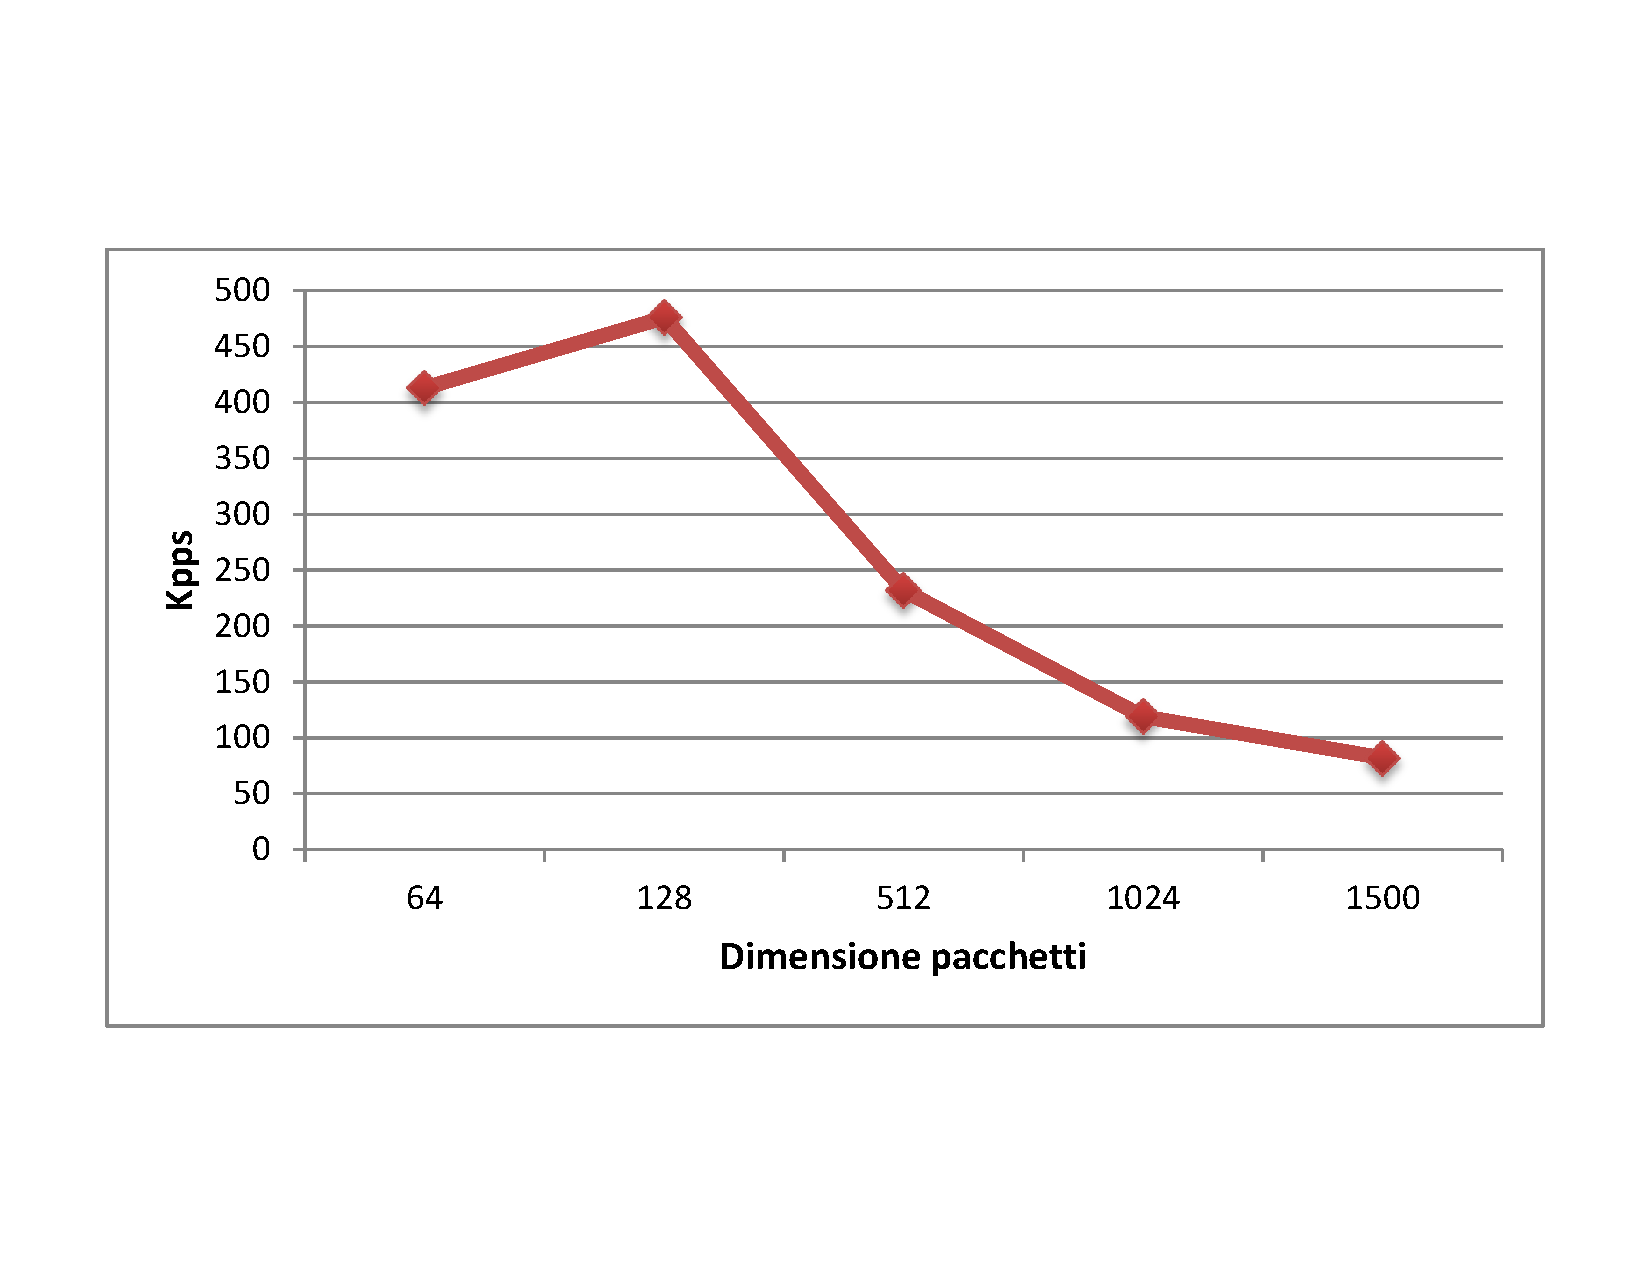
\includegraphics[scale=0.5]{img/kpps.pdf}
\caption{Capacità elaborativa di 4 thread \emph{monitor}}\label{kpps}
\end{center}
\end{figure}

\clearpage
A questo punto, per valutare il numero contemporaneo di sessioni tracciabili al secondo, si è usato un indice massimo di perdita di eventuali informazioni relativamente ad esse, aumentandole via via. Mantenendo il rate trasmissivo ancora a 1 Gbps, 4 thread \emph{monitor}, e la dimensione dei pacchetti a 512 byte, si sono ottenuti risultati davvero ottimi, mostrati nel grafico \ref{sess} seguente.

\begin{figure}[H] % htbp
\begin{center}
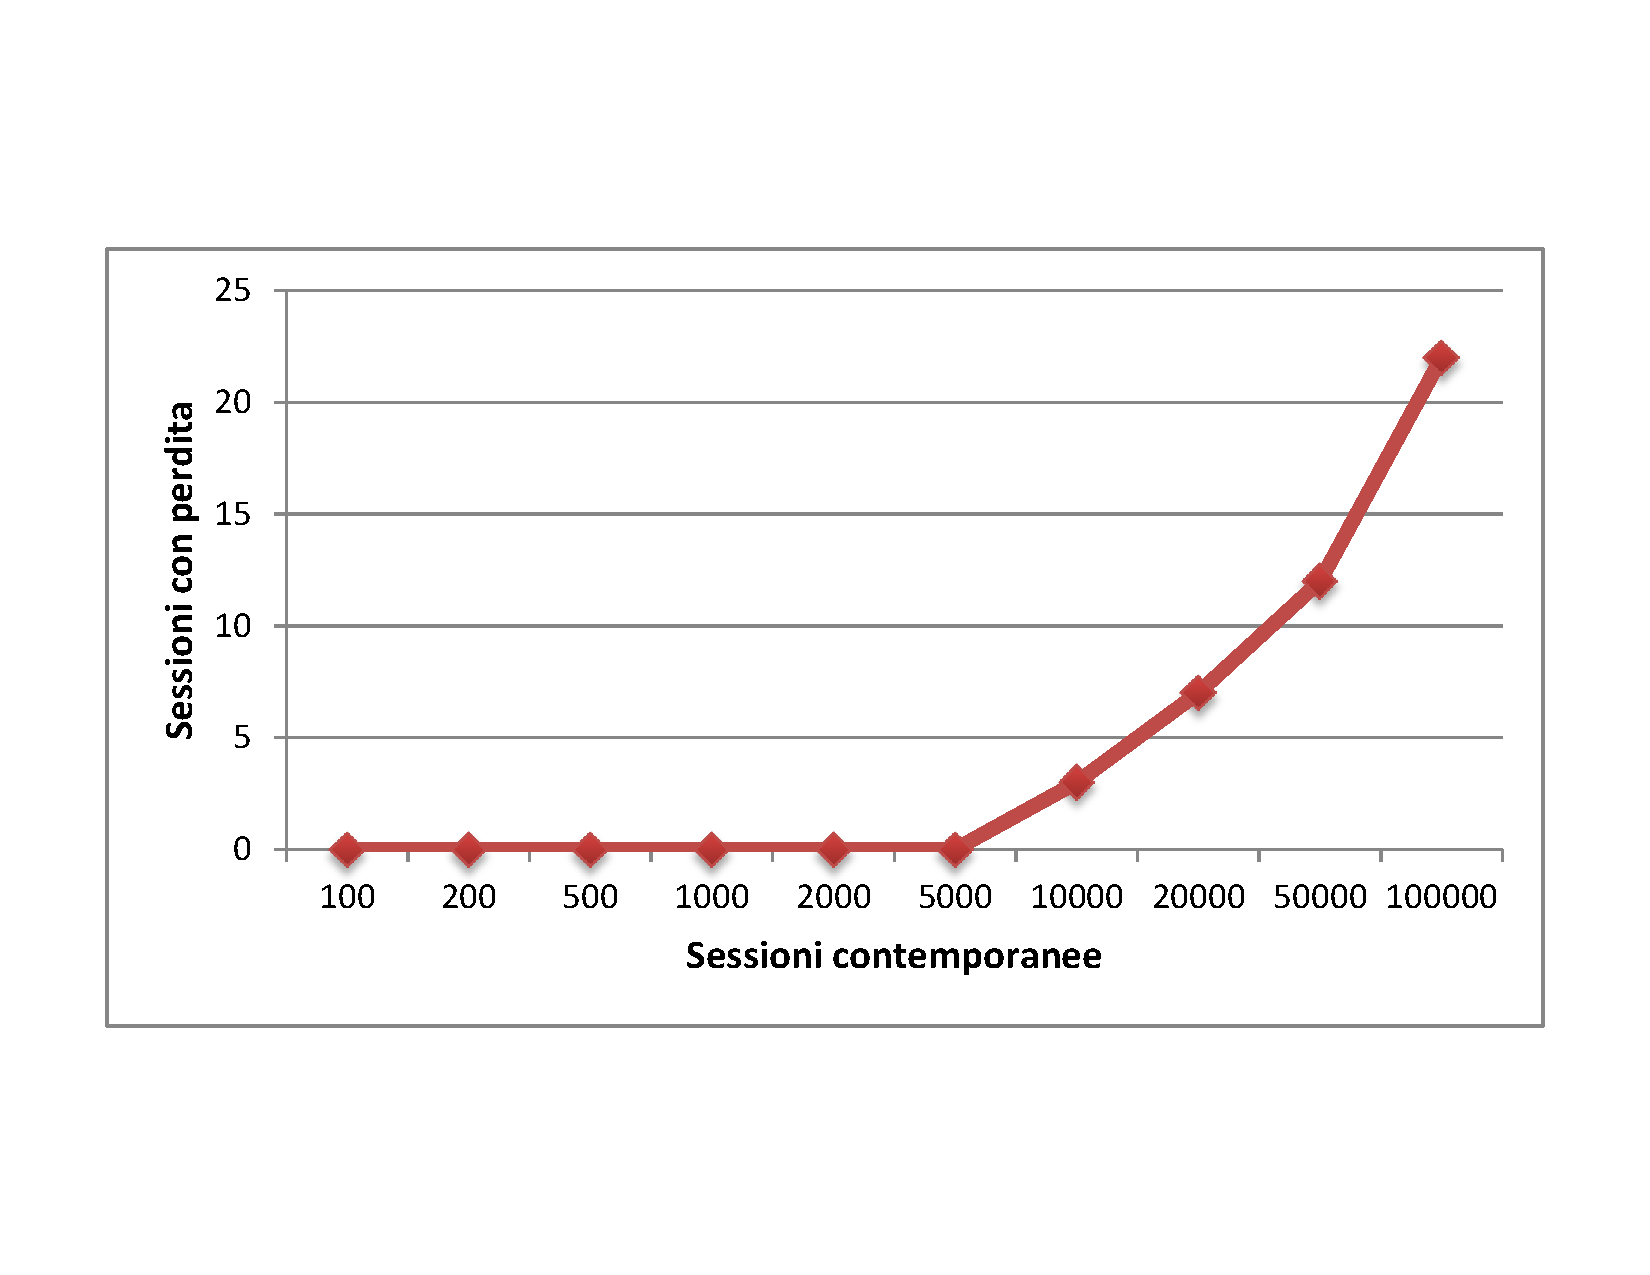
\includegraphics[scale=0.5]{img/sess.pdf}
\caption{Perdite su sessioni contemporanee}\label{sess}
\end{center}
\end{figure}

\clearpage
L'ultimo e più importante aspetto considerato, è stato quello del numero di migliaia di pacchetti processabili all'aumentare dei thread \emph{monitor} utilizzati. Questo è stato effettuato iniettando traffico reale limitato alla dimensione di 512 byte il pacchetto. I risultati, davvero ottimi, sono sintetizzati nel seguente grafico \ref{perf}.

\begin{figure}[H]
\begin{center}
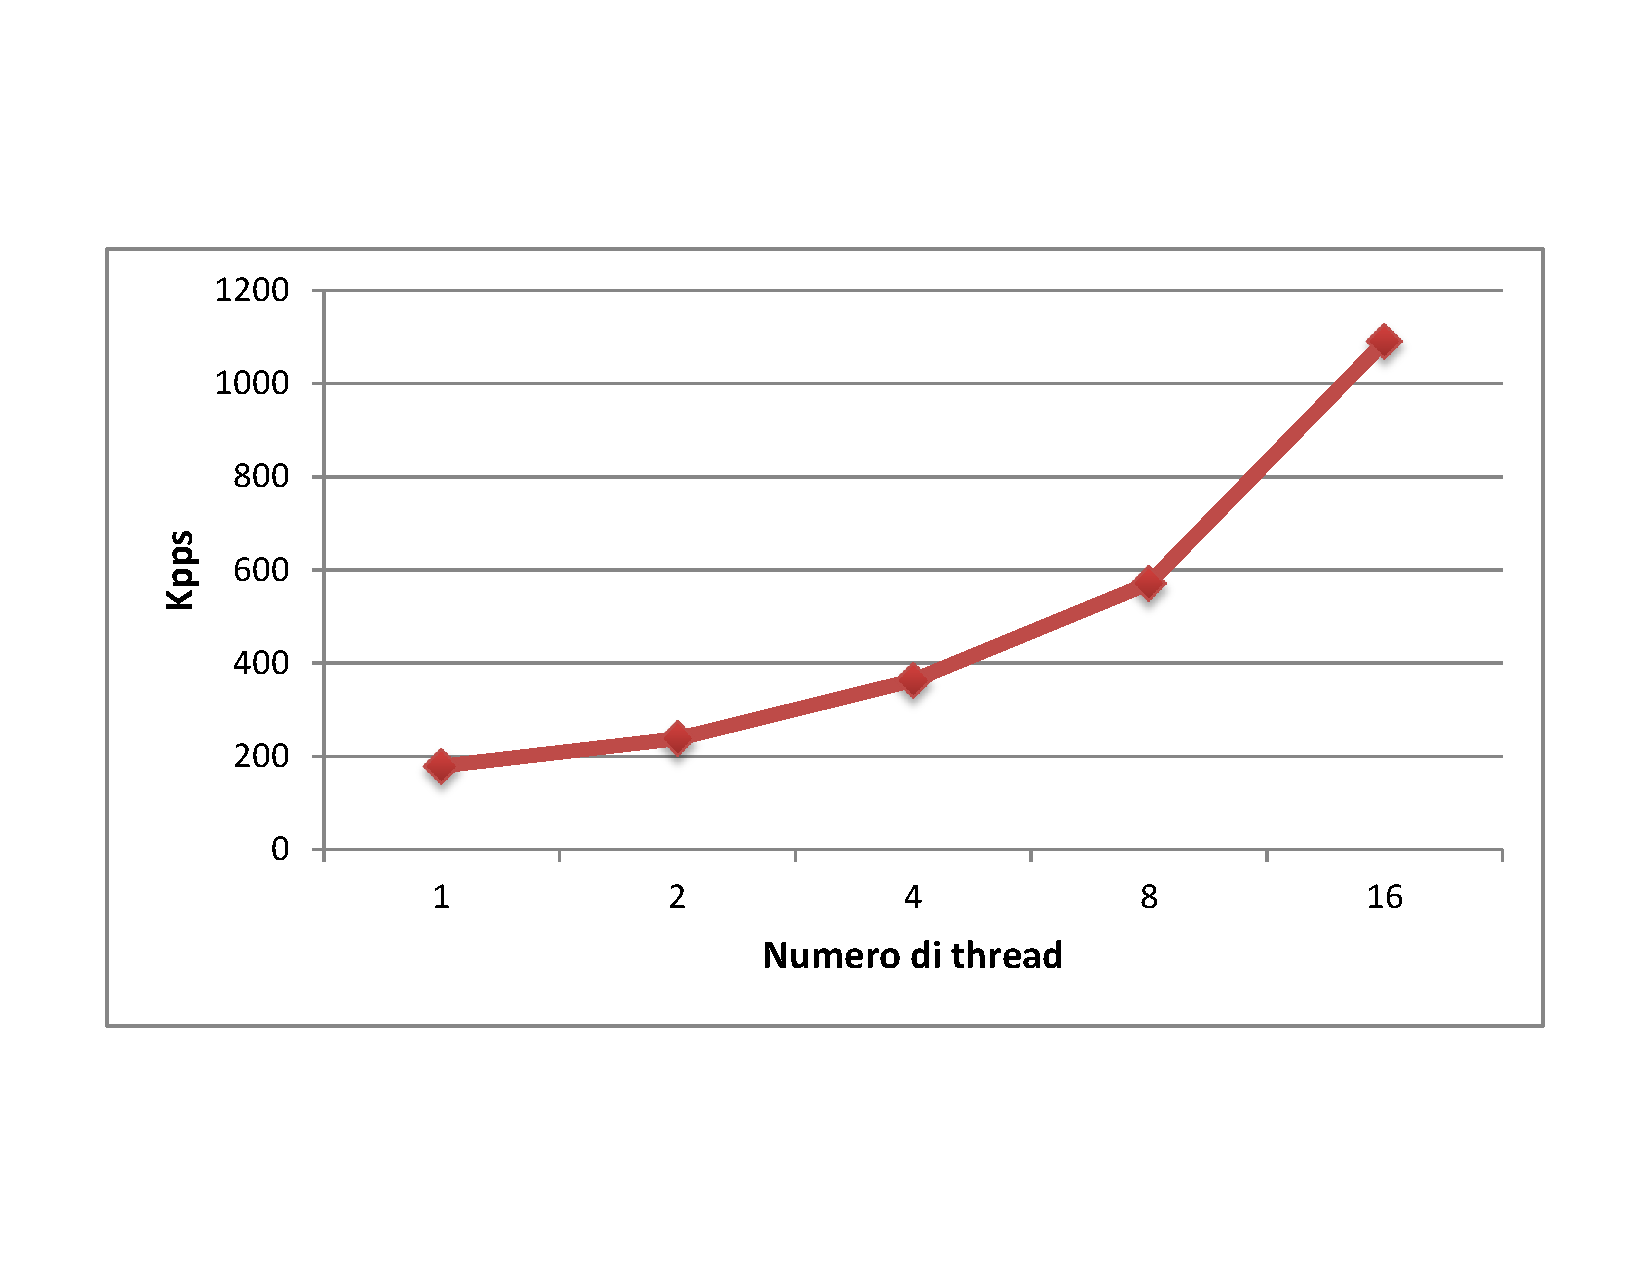
\includegraphics[scale=0.5]{img/perf.pdf}
\caption{Performance reali dell'applicazione}\label{perf}
\end{center}
\end{figure}

I risultati dei vari test sono dunque incoraggianti per lo sviluppo futuro e perfettamente in linea, se non superiori, con gli obiettivi prestabiliti.

Si ritiene comunque utile e doveroso eseguire test approfonditi sul software anche in base ai criteri stabiliti dalla RFC 3511 \cite{rfc3511}, riguardante la \emph{Metodologia di Benchmarking per le Performance dei Firewall}, al fine di ottenere dei dati oggettivi e standardizzati per una futura versione di rilascio.
\clearpage{\pagestyle{empty}\cleardoublepage}
\chapter{Related Work}

\section{Soluzioni per il DPI}

\subsection{Ipoque PACE}

PACE (\emph{Protocol and Application Classification Engine}) \cite{pace} è il motore DPI proprietario della Ipoque, mantenuto aggiornato per i servizi odierni.

Viene distribuita come libreria (statica e dinamica) realizzata interamente in C da utilizzare in user space, ma anche come modulo del kernel.

Naturalmente è compatibile con piattaforme a 32 e 64 bit, architetture Little e Big Endian, sia con sistema operativo Linux che Windows.

Per eseguire i compiti propri del DPI, sfrutta anche il pattern matching e analisi comportamentali, statistiche ed euristiche.

Grazie a questa combinazione di funzionalità, permette di riconoscere anche protocolli applicativi proprietari, cifrati e offuscati. Inoltre ha un tasso molto basso di falsi negativi, e praticamente nessun falso positivo.

I dettagli del codice chiaramente non sono visibili, ma dalle caratteristiche dichiarate della casa produttrice si ha che sono impiegati in media meno di 2000 cicli di clock per identificare un protocollo. La libreria nDPI (che ricordiamo basarsi sulle ceneri della versione free di questa libreria) invece ne impiega circa meno della metà, garantendo quindi migliori performance.

Sono fornite anche funzionalità per il tracking dei flussi di comunicazione (seppur se ne possano usare di proprie), che permettono di estrarre informazioni quali il \emph{Round Trip Time}. Stando a quanto dichiarato dalla Ipoque, consumerebbero in media meno di 1000 cicli di clock. Questo compito è assolto dalla flowHashTable, che però utilizza intorno ai 330 cicli di clock in media, garantendo quindi performance tre volte migliori.

Quindi, complessivamente, PACE impiega mediamente 3000 cicli di clock, mentre la soluzione adottata circa 1200. Ne consegue quindi che quest'ultima è decisamente migliore in termini di consumo di risorse del processore.

Infine questa libreria viene dichiarata come funzionante per reti operanti a velocità di 10 Gbit/s e oltre.

\subsection{Qosmos ixEngine}

ixEngine \cite{ixe} è il motore per il DPI e l'estrazione di metadati della Qosmos. Costruita a blocchi, permette facilmente l'integrazione con nuove o vecchie soluzioni. Grazie a questa caratteristica permette la scrittura di plugin, mediante un software scritto dalla ditta stessa.

L'aggiornamento quindi risulta piuttosto semplice ed è garantito giornalmente e on-demand dalla ditta.

I metadati estratti in tempo reale riguardano ad esempio tipo di file scaricato, IMSI, \dots

Una caratteristica importante di questa soluzione è che permette analisi anche su pacchetti frammentati, mentre la libreria nDPI non lo permette.

Essendo pensata per gestire grosse quantità di dati e l'operatività su reti a 10 Gbit/s, è stata ottimizzata per essere scalabile fino a 96 cores. 

Nonostante sia ottimizzata soprattutto per garantire ottime performance su piattaforme multicore (quali Cavium, Tilera e NetLogic), è comunque compatibile con le CPU prodotte dalle aziende leader di mercato, poiché sviluppata in C.

Supporta distribuzioni Linux con kernel 3.x, su piattaforme a 32 o 64 bit.

Purtroppo in questo caso non sono note le performace di tale libreria. Risulta quindi difficile fare veri e propri confronti con la libreria nDPI.

Viste però le importanti collaborazioni (con ad esempio anche Intel) si ritiene che questa libreria sia ben sviluppata.

\subsection{L7-Filter}

L7-Filter \cite{l7filter} è l'unico dei motori DPI open source degno di nota.

Viene spesso utilizzato come modulo del kernel in distribuzioni Linux specializzate per la gestione di rete (come ZeroShell, Zentyal, Untangle).

C'è comunque una versione beta per l'utilizzo in user space.

Per tentare di riconoscere il protocollo applicativo trasportato, L7-Filter analizza, mediante espressioni regolari, i primi 10 pacchetti di ogni nuova connessione (o  2 kByte di dati). Se l'utente volesse modificare tale limite, dovrebbe agire sul file \emph{layer7\_numpackets} nella directory \mbox{/proc/net/}.

Questa è una buona caratteristica, ma la libreria nDPI non ha di suo un vero e proprio limite (ricordiamo comunque che una volta stabilito il protocollo trasportato, i successivi pacchetti di quel flusso, se analizzati, sarebbero subito riconosciuti senza ulteriori operazioni, ma pagando comunque l'\emph{overhead} di una chiamata a funzione). Per garantirne uno, al fine di diminuire il numero di controlli che altrimenti dovrebbero essere effettuati dal firewall, si è scelto quindi di facilitare la cosa all'utente semplicemente permettendogli di impostarlo tramite riga di comando dell'eseguibile di \emph{L7-Bridge}.

Il problema principale di questa libreria è l'uso di pattern (cioè, nome del protocollo ed espressione regolare da ricercare) per il riconoscimento di un protocollo. Se da una parte questo semplifica la scrittura di nuove regole (caratteristica piuttosto importante, così da garantire facilità nell'estensione ed aggiornamento dei protocolli riconoscibili), dall'altra crea una buona possibilità di falsi positivi nel controllo dei pacchetti.

Quest'ultimo non è un problema da poco. Si potrebbe infatti gestire un certo flusso con una regola errata, ad esempio bloccandolo seppur in realtà sarebbe acconsentito, oppure, peggio ancora, consentire ad un servizio malevolo (\emph{virus}, \emph{backdoor}) di agire.

Una buona libreria DPI dovrebbe quindi limitare il più possibile questo aspetto, cruciale per il buon funzionamento del firewall in generale.

In questo caso, la libreria nDPI è da preferire in quanto, attraverso le proprie funzioni C, riduce al minimo le possibilità di falsi positivi.

L7-Filter in versione modulo del kernel, come anche nDPI, non ha funzionalità di tracking delle connessioni. Bisogna quindi affiancarci una qualche struttura dati per farlo. Per quanto riguarda la beta per user space invece è presente una minimale struttura dati preposta a questo scopo, ma è stata utilizzata la \emph{map} (sostanzialmente, una hash table) fornita dalle librerie standard del C++ con diverse sezioni critiche gestite con meccanismi di sincronizzazione (lock/unlock), quindi con notevole degrado delle performance.

In \emph{L7-Bridge} è stata creata ad hoc ed utilizzata la flowHashTable per questo scopo, con ottimi risultati.

A livello di performance, viene raccomandato l'uso di L7-Filter su macchine che devono gestire al più 5000 pps (pacchetti per secondo) \cite{gheorghe}, ovvero su Megabit LAN. Questa caratteristica la rende quindi inutilizzabile sulle reti Gigabit Ethernet moderne, che sono il target del progetto \emph{L7-Bridge}.

\section{Soluzioni per il Traffic Shaping}

\subsection{MasterShaper}

MasterShaper \cite{ms} fa parte di quei software open source che sfruttano il \emph{traffic control} di Linux al fine di effettuare lo shaping dei servizi.

Come già detto in precedenza, questi meccanismi non sono alla portata di tutti, quindi MasterShaper offre ai suoi utenti una comoda interfaccia web per guidarli nelle varie impostazioni. Questa scelta è piuttosto apprezzabile, in quanto sempre più spesso si ha familiarità con i browser.

Per la configurazione del \emph{trafficShaper} di \emph{L7-Bridge} invece, è stato scelto di far impostare dall'utente un file XML contenente le specifiche delle varie code di priorità da creare. Questo potrebbe risultare meno immediato rispetto ad un'interfaccia web come quella di MasterShaper, ma la semplicità con cui è possibile scrivere il file di regole, magari tramite l'ausilio del proprio editor XML preferito, non dovrebbe farla rimpiangere troppo.

Oltre che per impostare le proprie preferenze, l'utente può sfruttare l'interfaccia web per avere grafici ed informazioni sul traffico in tempo reale. Quest'ottima funzionalità non è al momento implementata in \emph{L7-Bridge}, ma si prevede di fornirla al più presto.

Fra le varie funzionalità è presente la possibilità di integrare L7-Filter come motore d'analisi DPI per effettuare lo shaping in base ai protocolli applicativi. Questo è un altro punto a favore di questo software.

Il problema critico che però si porta dietro lo sviluppo di questo progetto è la dipendenza dal kernel di Linux e anche dai diversi pacchetti supplementari di cui ha bisogno per funzionare (come \emph{iproute2}, package di utility per il networking, che contiene il fondamentale comando \emph{tc}, che permette di manipolare le code di priorità dei pacchetti proprie del kernel).

In pratica ad ogni modifica (e sappiamo che i kernel di Linux cambiano frequentemente), i comandi da impartire tramite \emph{tc} potrebbero dover andar rivisti, con conseguente bisogno di rilascio di patch o nuove versioni del software.

Da queste semplici considerazioni si capisce come sia necessario mantenere lo shaping separato dai vari aspetti del kernel. In questo senso, lo shaper realizzato in \emph{L7-Bridge} è del tutto indipendente da ogni altro componente del sistema operativo, garantendo così la possibilità di non dover essere la preoccupazione numero uno per lo sviluppo del progetto.

\subsection{Trickle}

Trickle \cite{trickle} è una libreria operante in spazio utente, senza che si abbia bisogno di particolari privilegi, che si interpone tra le chiamate a system call quali send, recv, \dots, ritardandone la loro effettiva esecuzione da parte del sistema operativo. Così facendo si realizza un naturale shaping della banda di una qualsiasi applicazione.

Questa interposizione è ottenuta grazie a LD\_PRELOAD che permette di caricare prima questa libreria dinamica rispetto alla standard \emph{libc.so}, utilizzata per garantire varie funzionalità sui socket BSD di rete.

Può essere eseguita su sistemi operativi Linux, FreeBSD, e Solaris, che supportano il preload delle librerie. Ha inoltre bisogno della \emph{libevent} \cite{libevent}, su cui poggia per assolvere al proprio compito.

Quest'ultima è una libreria di notificazione degli eventi asincroni che fornisce un meccanismo per eseguire una funzione di callback quando su un descrittore di file avviene un determinato evento o dopo che è scaduto un timeout. Venne ideata al fine di sostituire l'event loop asincrono nei server di rete pilotati da eventi. Attualmente, \emph{libevent} gestisce importanti system call quali /dev/poll, kqueue, event ports, select, poll, e epoll. Essendo indipendente dall'event API esposta, è possibile garantire nuove funzionalità con semplici aggiornamenti, senza dover riprogettare le applicazioni. Inoltre è utilizzabile anche in programmi multi-threaded.

Da tutte queste premesse si capisce come Trickle sia facilmente portabile, aggiornabile e soprattutto non abbia alcun problema coi kernel di Linux. Inoltre lo shaping di una applicazione avviene con semplici ed intuitivi comandi impartibili via riga di comando (es.: \mbox{trickle -d 50 -u 10 \emph{applicazione},} dove con -d si limita il download e con -u l'upload dell'applicazione, e quindi la socket, specificata). Esiste anche \emph{trickled}, un demone di sistema di Trickle che permette di fare lo shaping di tutte le socket aperte, sempre con le stesse modalità d'uso.

Questo aspetto fa propendere l'uso di Trickle per singoli host, cioè dove è presente una socket per ogni applicativo che apre un flusso di comunicazione. Con qualche modifica, sarebbe però possibile adattarlo al fine di farlo funzionare anche su macchine facenti da bridge o firewall in generale.

Purtroppo questa libreria soffre di alcuni importanti problemi generali.

Innanzitutto, Trickle opera solo su connessioni TCP, anche se questo è il protocollo di trasporto più usato per i servizi Internet.

Per la sua natura, Trickle è in grado di limitare solo applicazioni utilizzanti librerie dinamiche. Se invece l'implementazione di un servizio usasse librerie statiche, non sarebbe possibile attivare le funzionalità di shaping.

Infine, ogni impostazione è da impartire tramite shell, quindi non è possibile stabilire delle vere e proprie politiche di utilizzo della banda, se non tramite comandi espliciti.

Date tutte queste caratteristiche, non è perfettamente integrabile nel firewall \emph{L7-Bridge}.

C'è bisogno di effettuare lo shaping indipendentemente dal protocollo di trasporto utilizzato, e il \emph{trafficShaper} adottato risponde perfettamente a questa prerogativa.

Le \emph{masterQueue} del \emph{trafficShaper} implementato sono astrazioni che permettono di definire delle politiche d'uso della banda, caratteristica desiderabile di ogni shaper.

L'aspetto invece desiderabile che ha Trickle nei confronti del \emph{trafficShaper} di \emph{L7-Bridge} è l'assenza di meccanismi di sincronizzazione.

\subsection{QFQ : Quick Fair Queueing}

QFQ \cite{qfq} è un packet scheduler appartenente alla categoria degli \emph{Approximated Fair Queueing schedulers}. Attualmente è utilizzato anche nell'importante progetto Dummynet \cite{dummynet}.

Questi scheduler hanno la proprietà di avere una piccola deviazione per flusso di comunicazione rispetto al tempo ideale di servizio. La componente che influenza di più questo scostamento è inversamente proporzionale alla banda richiesta dal flusso. Anche se godono di una complessità di tempo nell'ordine di O(1) nel numero di flussi, sono diverse volte più costosi rispetto agli scheduler di tipo Round Robin, che però non danno praticamente alcuna garanzia sulla deviazione. Quest'ultimo tipo di scheduler è stato utilizzato nei principi per l'implementazione del \emph{trafficShaper}, che gode quindi di tutte le relative caratteristiche.

QFQ ha l'interessante proprietà di avere complessità di O(1), dando garanzia quasi ottimale sulla deviazione per flusso.

Per fare questo, sfrutta le basi teoriche proprie della categoria di scheduler alla quale appartiene, ma usa nuovi meccanismi per rimuovere il costo lineare nel numero di gruppi di flussi, o lunghezza dei pacchetti, caratteristici dei precedenti quasi-O(1) schedulers.

In QFQ, i flussi sono divisi in quattro gruppi, ciascuno rappresentato da una parola (\emph{word machine}). Questa è costruita in modo tale che tutte le informazioni necessarie a far prendere le decisioni allo scheduler possano essere effettuate utilizzando istruzioni semplici e costanti in tempo d'esecuzione, come AND, OR, XOR e trovare il primo bit a 1 (\emph{Find First Set bit}), utilizzata per implementare in tempo costante la ricerca del prossimo gruppo da servire.

L'implementazione del \emph{trafficShaper} in Round Robin invece, non necessita di tali strutture dati. Basta semplicemente utilizzare un indice della successiva coda da servire, ottenendo quindi tale informazione con una singola istruzione.

Grazie a questi accorgimenti, e ad un algoritmo che non ha bisogno di alcun ciclo, QFQ ha davvero delle ottime performance, dichiarate nell'ordine del centinaio di nanosecondi per coppia di enqueue()/dequeue().

Il \emph{trafficShaper}, realizzato seguendo i principi del Deficit Round Robin, è comunque ancora più veloce da questo punto di vista, impiegando qualche decina di nanosecondo in meno, ma con minori garanzie sulla deviazione rispetto al tempo ideale di servizio.

Bisogna però dire che in realtà il \emph{trafficShaper} deve utilizzare meccanismi di sincronizzazione che ne degradano le performance rispetto a quelle suddette. Questo aspetto però non è valutato nei test effettuati su QFQ, forse perchè più pensato per l'uso come modulo del kernel, che non in user space.

\section{Soluzioni per firewall applicativi}

\subsection{Netfilter}

Netfilter \cite{netfilter} è un framework che permette l'interazione col modulo kernel di Linux per l'intercettazione e la manipolazione dei pacchetti ricevuti. Col tempo è diventato un componente standard di tutte le moderne distribuzioni di Linux. L'ultima release stabile è quella basata sulla versione 3.1 del kernel.

Netfilter permette di realizzare alcune funzionalità di rete avanzate come l'implementazione del servizio di NAT (\emph{Network Address Translation}), e quindi la condivisione di un'unica connessione Internet tra diversi computer di una rete locale.

Comprende diversi tool specializzati per svolgere tante e diverse funzioni di rete, in continua espansione ed interagenti tra loro. Tale aspetto può essere interpretato come un pregio, ma anche come un difetto.

Un esempio dei vari strumenti disponibili è iptables, che permette di definire le regole per i filtri di rete ed è progettato per poter essere facilmente esteso attraverso moduli che aggiungono funzionalità.

Come si evince quindi, è l'accoppiata Netfilter e iptables che permette la creazione di firewall.

Per aggiungere le funzionalità proprie del DPI, si utilizza un modulo di iptables derivato da L7-Filter.

Ne consegue che qualsiasi firewall si crei, sarà sempre affetto dalla possibilità di falsi positivi e dalle ridotte performance.

Per raccogliere statistiche basate sui flussi di comunicazione, è necessario un altro tool della suite, conntrack-tools. Quest'ultimo ha caratteristiche interessanti, come la possibilità di visualizzare le informazioni collezionare in testo semplice o XML e definire i timeout per gli aggiornamenti ed eliminazioni delle varie connessioni tracciate.

Solo con Netfilter e iptables, non sarebbe possibile effettuare l'importante funzionalità di traffic shaping.

Per poterla permettere c'è bisogno dell'uso di \emph{tc}, per manipolare il \emph{traffic control} di Linux.

Una soluzione basata su questi tool mostra evidenti problemi.

Il primo che salta subito agli occhi è la dipendenza dal kernel di Linux. Questo potrebbe significare il dover mantenere sempre aggiornati tutti i vari strumenti, che inoltre hanno qualche dipendenza tra loro. Da un altro punto di vista, certe funzionalità potrebbe comunque essere limitate dal kernel stesso. Insomma, un firewall basato sul framework di Netfilter potrebbe avere diversi problemi di manutenibilità.

\emph{L7-Bridge} mantiene ben separati i vari moduli del sistema, permettendo una facile manutenzione ed aggiornamento.

Da non sottovalutare anche la difficoltà nella configurazione del firewall. I tanti tool da dover utilizzare per realizzare un firewall completo possono far creare confusione.

\emph{L7-Bridge} invece permette con un solo semplice file XML l'intera configurazione del sistema.

Nonostante questi aspetti, diversi validi prodotti software sono presenti sul mercato, un esempio di essi è Shorewall (Shoreline Firewall).

\subsection{pfSense}

pfSense \citep{pfsense} è un potente firewall software open source basato su FreeBSD.

Incorpora varie funzionalità, da quelle più semplici a quelle più complesse.

Per fare qualche esempio, ricordiamo le funzionalità di NAT (\emph{Network Address Translation}), la possibilità di bilanciare il carico di lavoro tra due o più server che si trovino dietro pfSense, l'affidabilità garantita grazie al modulo CARP e pfsync (permette di configurare due firewall su due macchine identiche per replicarsi e autosostituirsi nel caso di guasto di una delle due), la gestione di uPnP, DHCP, Dynamic DNS, e molte altre. Inoltre è possibile visualizzare e salvare varie statistiche sui flussi della rete.

Insomma, si tratta di un software veramente completo.

Nello specifico \emph{L7-Bridge} non presenta tutte queste caratteristiche, in quanto comunque è ancora un progetto giovane.

I due firewall sono però comparabili in alcune caratteristiche (come l'uso di un file XML per la configurazione) e nelle funzionalità essenziali, quali la possibilità di analizzare approfonditamente i pacchetti per stabilire il protocollo applicativo trasportato e effettuare lo shaping del traffico.

Per effettuare il DPI dei pacchetti, pfSense utilizza \emph{ipfw-classifyd}, sostanzialmente basato su L7-Filter, mentre per lo shaping si appoggia a Dummynet (e quindi implicitamente a QFQ).

Avendo già analizzato entrambe le componenti sono noti i pro e i contro della soluzione.

Nello specifico, mentre Dummynet è comunque una buona scelta per lo shaping, l'uso di un motore d'analisi basato su L7-Filter si dimostra non essere l'alternativa migliore per il DPI (ricordiamo comunque come sia praticamente l'unica possibilità nel mondo open source). Sicuramente i requisiti hardware richiesti sono influenzati da quest'ultima scelta e non solo dalle notevoli funzionalità offerte da questo software.

\emph{L7-Bridge} invece, utilizzando nDPI, permette di analizzare maggiori quantità di pacchetti a parità di hardware, oppure, detta in altri termini, permette di analizzare lo stesso traffico con una macchina decisamente meno all'avanguardia (quindi meno costosa).

Infine, da un punto di vista di usabilità del software, c'è da considerare il fatto che pfSense permette anche di effettuare la gestione del firewall tramite interfaccia grafica web, cosa decisamente apprezzabile per l'utente, mentre, al momento, \emph{L7-Bridge} consente solo l'uso tramite riga di comando.

\subsection{SonicWALL Firewall}

La ditta SonicWALL \cite{sonicwall} produce firewall integrati in appositi apparati di rete con supporto al DPI e allo shaping.

Questo tipo di soluzioni godono di ottime performance, dovute al fatto che sfruttano dell'hardware dedicato. C'è anche la possibilità di modificare varie impostazioni e monitorare lo stato attuale del componente tramite un'intuitiva e semplice interfaccia web.

Il grosso contro è dovuto al prezzo.

La soluzione meno cara costa già oltre 350 euro (senza contare che bisogna pagarne ogni anno altri 200 per il rinnovo), ma gestisce traffico solo fino a 100 Mbps, davvero poco per reti ad alte velocità come quelle attuali.

Per ottenere un prodotto capace di gestire almeno 1 Gbps di traffico, si dovrebbe versare oltre 2500 euro con solo un anno di supporto dalla ditta.

Queste semplici cifre fanno riflettere sulla necessità di avere un firewall applicativo con le stesse funzioni.

In questo senso \emph{L7-Bridge} è in grado di fornire prestazioni analoghe con un PC standard. Inoltre, grazie alla semplicità d'estensione della libreria nDPI, è facilmente aggiornabile e l'utente può scrivere ed utilizzare le proprie funzioni per il riconoscimento dei protocolli.
\clearpage{\pagestyle{empty}\cleardoublepage}
\chapter{Conclusioni}

\section{Sviluppi futuri}

\subsection{Scan probabilistico per il DPI}

L'attuale implementazione della libreria nDPI è piuttosto buona, ma ha un paio di pecche.

La prima è che utilizza una struttura principale dove vengono salvate delle informazioni temporanee inutilmente (ad esempio il puntatore alla struttura che conserva le precedenti informazioni su un flusso). Così facendo, in ambiente multi-threaded è utilizzabile solo se replicandola per ogni thread o mettendo dei meccanismi di sincronizzazione. Se si riscrivesse il codice affinché ad ogni funzione (anche interna) vengano passati tutti i puntatori e valori di cui ha bisogno, si potrebbe facilmente evitare tale problema.

La seconda pecca, decisamente più rilevante rispetto alla precedente, riguarda il modo in cui vengono provate le funzioni che cercano di stabilire il servizio trasportato dal pacchetto. Ora come ora tale scan avviene in modo \emph{lineare}, ovvero dalla prima funzione del buffer in poi. Sarebbe però interessante provare a farlo diventare \emph{probabilistico}, cioè provare per prima quella del protocollo applicativo che è più probabile per quel tipo di pacchetto. Ad esempio, sapendo che DNS usa UDP con porta 53, se ci si trova ad esaminare un pacchetto con queste caratteristiche, la prima funzione da applicare sarebbe quella del servizio DNS e poi eventualmente tutte le altre.

\subsection{Velocizzare il tracking dei flussi}

Sicuramente è la struttura dati più interessata, dovendo essere utilizzata per ogni pacchetto ricevuto.

Nonostante sia stata sviluppata con particolare cura per i dettagli, e seppur i test abbiano già dato ottimi risultati, c'è sempre del margine di miglioramento, anche se per pochi cicli di clock.

Dal punto di vista algoritmico e dello spazio occupato in memoria probabilmente si possono fare ben pochi aggiustamenti.

Dal punto di vista computazionale invece, c'è la possibilità di limare ancora qualche ciclo di clock, che per milioni di pacchetti potrebbe comunque dir tanto in termini di performance.

Si prevede in tal senso di utilizzare istruzioni \emph{Streaming SIMD Extensions} (SSE) \cite{sse}. Con l'ausilio di quest'ultime, ad esempio il calcolo dell'hash risulterebbe fatto con una singola istruzione, offrendo quindi la possibilità di un ulteriore aumento delle performance.

\subsection{Migliorie alla gestione delle regole}

Attualmente le regole vere e proprie vengono salvate in una semplice lista, poiché il miglior modo di gestire un firewall è quello di averne sempre un numero contenuto, in accordo anche con quanto detto in \cite{fsr}.

Nonostante questo abbia un fondo di verità, è anche vero che nessuno può impedire a grosse organizzazioni di avere un elenco di regole immenso.

A seguito di questa considerazione, si potrebbe gestire le regole tramite una hash table, anziché una sola lista, garantendo migliori performance in fase di creazione (notiamo che questo non influirebbe nella fare di ricerca, in quanto l'accesso avverrebbe sempre tramite l'albero binario).

Si prevede anche di provare l'implementazione dell'albero di Patricia con il supporto dell'hash \cite{hpt,hat}, ipotesi che per questa versione del software era stata accantonata.

\subsection{Lockless shaping}

Il trafficShaper costituisce l'unico esempio in cui sono stati utilizzati i meccanismi di sincronizzazione. Questo significa che è un elemento di degrado delle performance.

Si ha quindi intenzione di migliorarlo facendo in modo che ogni thread \emph{monitor} abbia una propria coda dove inserire i propri pacchetti da inviare, così da non dover più utilizzare alcuna lock/unlock.

Per ora questo approccio ha un problema irrisolto, cioè garantire che sia comunque rispettato l'ordine di arrivo all'interno di ogni \emph{masterQueue}, ovviamente in modo efficiente.

Quando si usa un'unica coda, questo avviene immediatamente dall'ordine con cui i pacchetti sono inseriti. Purtroppo dividendola su più sotto-code, questa assunzione non è più valida.

Ovviamente eseguire dei controlli incrociaci su ogni pacchetto in testa ad ogni sotto-coda non sarebbe per nulla efficiente.

Quando sarà trovata soluzione a questo problema, sarà modificato il modulo che gestisce lo shaping.

\subsection{Il prossimo passo per L7-Bridge}

Attualmente per catturare i pacchetti è utilizzata la libreria PF\_RING.

Da qualche tempo è però stata sviluppata e rilasciata una nuova libreria nata dal ramo DNA dalla precedente, si sta parlando di \emph{libzero} \cite{libzero}.

Quest'ultima permetterebbe di ovviare al problema dell'esecuzione del software in zero-copy del pacchetto, essendo studiata appositamente a questo scopo (come suggerisce il nome), garantendo così performance ancora migliori delle attuali.

L'implementazione adottata inoltre permette di passare a questa nuova tecnologia praticamente a costo zero, infatti ciò che viene ora passato ai vari thread \emph{monitor} è un puntatore ad una struttura contenente un buffer per il pacchetto (che sostanzialmente è un puntatore alla sua copia). Basta quindi sostituire questo buffer con il puntatore al pacchetto vero e proprio.

Da un punto di vista estetico, ma anche e soprattutto funzionale, si prevede di fornire un'interfaccia grafica via web con la quale poter configurare l'intero sistema e visualizzare grafici e varie informazioni in tempo reale sul traffico che il bridge sta processando in quel momento, nonché dei log riguardanti problemi registrati durante le operazioni. Questo sia a fini di monitoraggio che di sicurezza della rete.

Dato l'aspetto modulare del sistema, le capacità d'espansione sono pressoché illimitate. Ad esempio si prevede l'inserimento di un modulo per impedire l'\emph{arp poisoning}, uno per impostare filtri \emph{antispam}, e uno per il \emph{fingerprinting} dei sistemi che usano la banda.

\section{Competenze acquisite}

Grazie all'esperienza maturata nel progettare e sviluppare questo software, è stata acquisita grande sensibilità nei confronti delle tecnologie utilizzabili per effettuare monitoraggio di reti, sia a livello di cattura che di analisi del traffico.

Dal punto di vista computazionale è emerso come i costi delle istruzioni, seppur singole e apparentemente semplici, possano garantire le migliori performance possibili (anche perché sono comunque eseguite potenzialmente per ogni pacchetto, e avendone milioni da processare, fanno veramente la differenza). Ad esempio, c'è notevole differenza in termini di istruzioni macchina per effettuare un'operazione di \emph{modulo} rispetto alla stessa funzione fatta attraverso un \emph{if}.

Si è potuto constatare come l'utilizzo dei thread possa far aumentare le capacità di calcolo, ammesso che la loro esecuzione sia veramente disgiunta. Nello specifico, per esempio, evitare meccanismi di sincronizzazione, può far aumentare notevolmente le performance.

Inoltre si è potuto constatare come l'utilizzo di appropriate strutture dati e algoritmi possa davvero fare la differenza in fase d'esecuzione, garantendo immediatezza nella ricerca delle informazioni.

\section{Conclusioni}

Si è realizzato un ottimo firewall applicativo di nuova generazione.

Dando uno sguardo in concreto ai risultati ottenuti, si può notare come con un semplice PC, acquistabile per qualche centinaia d'euro, sia possibile gestire volumi di traffico intorno al Gigabit/s.

Dal punto di vista progettuale, si ritiene che il software sia ormai maturo per un imminente rilascio, grazie anche all'intensa attività di test, che ha dato ottime conferme fin da subito e buoni auspici per il proseguo dello sviluppo.

\emph{L7-Bridge} fornirà agli amministratori di rete un nuovissimo strumento, facilmente configurabile, per effettuare tutte quelle operazioni possibili solo con la congiunzione tra DPI e shaping, e che ora sono praticabili solo con soluzioni proprietarie costose, talvolta anche difficilmente gestibili.

Ovviamente è stato concepito per le reti attuali, ma ha ottime caratteristiche che lo rendono facilmente aggiornabile per rimanere sempre al passo coi tempi.

\clearpage{\pagestyle{empty}\cleardoublepage}
\phantomsection
\addcontentsline{toc}{chapter}{\bibname}
\bibliography{bibliografia}


\appendix
\clearpage{\pagestyle{empty}\cleardoublepage}
\addtocontents{toc}{\protect\addappendixname}
\chapter{Dove reperire il codice}

Allegare qui tutti i sorgenti creati sarebbe inutile e tedioso.\\

Attualmente il codice è mantenuto via SVN, ed è quindi preferibile dare il riferimento dell'indirizzo web per chi volesse scaricarlo e provarlo\\

\url{https://svn.ntop.org/svn/sgr/2012/lipilini/l7-bridge}\\

Si prevede però di rilasciarlo presto tramite l'ausilio di siti preposti, come \mbox{SourceForge}, sotto la classica licenza GNU GPL per software open source.

\end{document}